\chapter{Higher Dimensional Systems}
\label{C:HDS}

\normalsize

In Chapter~\ref{chap:SolveOdes} we saw that equilibria and their 
stabilities completely determined the phase line dynamics for single
autonomous first order differential equations.  The stability of the
equilibria determine the direction in which one equilibrium is connected 
to the next.

In Chapter~\ref{C:NPS} we discussed the extent to which equilibria and 
their stability determined the phase planes of systems of two autonomous 
systems of ordinary differential equations.  When an equilibrium is 
hyperbolic, nonlinear planar systems behave much like their linearizations 
--- at least on a small neighborhood of the equilibrium.  However, away 
from equilibria, planar systems can have dynamically more interesting 
states: limit cycles.  We have seen that qualitatively we can understand the
global dynamics of most planar systems (the Morse-Smale ones) if we can find 
their equilibria, their periodic
solutions, and their connecting orbits.  Analytically, this is an impossible
problem to solve in closed form --- but numerically this kind of calculation
is often tractable.

In this chapter we discuss briefly the dynamics of systems of three or
more autonomous first order differential equations.  The situation is
very complicated --- even on the qualitative level.  On the positive
side, nonlinear systems do behave like their linear counterparts on a
neighborhood of hyperbolic equilibria, and the dynamics of the linearized
systems can be understood as a consequence of the Jordan normal form theorem.
These issues are discussed in Sections~\ref{sec:LinHomSys} and \ref{S:QT}.  
On the negative side, in Sections~\ref{S:NLD} and \ref{S:chaos} we will see 
that the dynamics of nonlinear systems away from equilibria are just much 
more complicated than their planar counterparts.  In particular, we will see 
that quasiperiodic motion may be expected (first in linear nonhyperbolic four 
dimensional systems and then in nonlinear three dimensional systems).  
Finally, we show that even complicated `chaotic' motion may be expected in 
three dimensions (the Lorenz equations). 

The discussion in Sections~\ref{S:NLD} and \ref{S:chaos} is predicated on 
being able to solve numerically systems of differential equations with more 
than two equations.  To do this, we must use the \Matlab differential 
equations solver {\tt ode45} directly.  We introduce this solver in 
Section~\ref{S:ode45} by solving certain one-dimensional differential 
equations.  In this section we also discuss how to store functions in \Matlab 
m-files.  In Section~\ref{S:ode45HD} we use {\tt ode45} to solve several 
sample differential equations in three and four dimensions, and we display 
the results using \Matlab graphics. 

The discussion in this chapter continues an important theme: what 
information can we learn about the dynamics and solutions of nonlinear 
systems of ordinary differential equations from numerical simulation.  
Indeed, what can mathematics say that will help in interpreting numerically 
obtained solutions?  We will see that even on the qualitative level, the 
situation is very complicated --- complicated enough to guarantee that closed 
form solutions are, in general, not an option.  It should be noted, however,
that closed form solutions do exist for many particular types of equations 
(not least of which are the linear constant coefficient systems).  In later
chapters we will discuss some of the techniques of integration that allow us
to solve certain special kinds of differential equations in closed form.


\section{Linear Systems in Jordan Normal Form}
\label{sec:LinHomSys}

In this section we discuss one method for finding 
closed form solutions\index{closed form solution} to 
linear constant coefficient systems of ODEs based on 
Jordan normal form\index{Jordan normal form}. Let  
\begin{equation}  \label{eq:linsys}
\dps\frac{dX}{dt} = AX,
\end{equation}
where $A=(a_{ij})$ is a constant $n\times n$ matrix and $X$ is an 
$n$ vector.  In Theorem~\ref{T:linODEsoln} of Chapter~\ref{Chap:Planar} 
we showed that the general solution\index{general solution} to 
\Ref{eq:linsys} is
\[
X(t) = e^{tA}X_0,
\]
where $X_0=X(0)$ is the initial condition\index{initial condition}.  
In Chapter~\ref{Chap:Planar} 
we used this theorem to solve planar systems of ODEs in closed form.
Now we apply matrix exponentials to solve \Ref{eq:linsys} for an 
arbitrary matrix $A$ --- at least in principle.
There were three ideas behind finding solutions to planar systems:
\begin{itemize}
\item[(a)] Exponentials\index{matrix!exponential} of similar 
matrices are similar\index{similar}.  More precisely,
\[
e^{P\inv AP} = P\inv e^{A}P,
\]
where $P$ is any invertible\index{invertible} matrix.  
See Chapter~\ref{Chap:Planar}, Lemma~\ref{L:similarexp}.
\item[(b)]	Every matrix $A$ is similar to a matrix in Jordan normal 
form --- in two dimensions the Jordan normal forms are
\[
B_1=\mattwo{\lambda}{0}{0}{\mu}, \quad B_2=\mattwo{\sigma}{-\tau}{\tau}{\sigma}
\AND B_3=\mattwo{\lambda}{1}{0}{\lambda}
\]
The first matrix corresponds to two 
real eigenvalues\index{eigenvalue!real} $\lambda$, $\mu$
with linearly independent eigenvectors; the second matrix 
corresponds to complex eigenvalues\index{eigenvalue!complex} 
$\sigma\pm i\tau$; and the third matrix is the only nontrivial 
Jordan block\index{Jordan block} in two dimensions.
\item[(c)]	It is possible to compute the exponentials of matrices in
Jordan normal form\index{Jordan normal form}.  Indeed,
\begin{eqnarray*}
e^{tB_1} &  = & \mattwo{e^{\lambda t}}{0}{0}{e^{\mu t}} \\
e^{tB_2} & = & 
e^{\sigma t}\mattwo{\cos(\tau t)}{-\sin(\tau t)}{\sin(\tau t)}{\cos(\tau t)} \\
e^{tB_3} & = &  e^{\lambda t}\mattwo{1}{t}{0}{1}.
\end{eqnarray*}
\end{itemize}

We use the same approach for solving linear systems in higher dimensions.
But in order to compute exponentials of matrices in Jordan normal form,
we need to verify one additional remark.

\begin{lemma}  \label{T:blocks}
Let the matrix $A$ be block diagonal, that is, let
\[
A=\mattwo{C_1}{0}{0}{C_2},
\]
where $C_1$ is a $\ell\times \ell$ matrix and $C_2$ is an 
$(n-\ell)\times(n-\ell)$ matrix.  Then 
\[
e^A = \mattwo{e^{C_1}}{0}{0}{e^{C_2}}.
\]
\end{lemma}

\proof  This lemma is proved by noting that
\[
A^k = \mattwo{C_1^k}{0}{0}{C_2^k},
\]
and applying the power series definition of matrix exponential.  
See Chapter~\ref{Chap:Planar}, \Ref{e:expL}. \qed

\subsection*{Matrix Exponentials of Jordan Normal Forms}

We compute matrix exponentials in two steps: first we consider 
Jordan blocks corresponding to real eigenvalues and second we consider
Jordan blocks with complex eigenvalues.  In this section we discuss mainly
solutions to linear systems already in Jordan normal form.  That is, we 
assume that a similarity transformation has already been performed that put
the coefficient
matrix into Jordan normal form.  In the next chapter, Section~\ref{S:SEOC},
we consider solving linear systems in their original coordinates. 

\subsection*{Real Eigenvalues}

A Jordan block with a real simple eigenvalue is just a $1\times 1$ matrix
$(\lambda)$. This matrix corresponds to the single equation 
$\dot{x}=\lambda x$ whose solution is $x(t) = e^{\lambda t}x_0$.

The $k\times k$ Jordan block\index{Jordan block} with real 
eigenvalue\index{Jordan block!with real eigenvalue} $\lambda$ is 
\[
\lambda I_k + N
\]
where the only nonzero entries in $N$ are the $1$s on the superdiagonal.  
Recall that \Ref{e:Ndef} in Chapter~\ref{C:HDeigenvalues} implies that 
$N^k=0$.  Since $I_k$ and $N$ commute, Proposition~\ref{P:expAB} of 
Chapter~\ref{Chap:Planar} implies that $e^{t(I_n+N)}=e^{tI_n}e^{tN}$.  We 
can compute the solution to the differential equation as:
\begin{eqnarray}
X(t) & = & e^{\lambda t}e^{tN}X_0 \nonumber \\
& = & e^{\lambda t}\left(I_k+tN+\cdots+\frac{1}{k!}t^{k-1}N^{k-1}\right)X_0.
\label{e:expsoln}
\end{eqnarray}

Note that $N^2$ is the matrix with $1$s on the second diagonal above the main
diagonal and $0$s elsewhere.  Similarly, $N^3$ is the matrix with $1$s on the 
third diagonal above the main diagonal and $0$s elsewhere, etc.
 

\subsubsection*{An Example of a Real Eigenvalue Jordan Block Equation}

Consider the case of a $k=3$ Jordan block with eigenvalue $\lambda=-0.5$.  
Then
\[
X(t) = e^{-0.5t} \left(\begin{array}{ccc} 1 & t & \frac{t^2}{2} \\
0 & 1 & t \\ 0 & 0 & 1 \end{array}\right)X_0.
\]
We can now solve the initial value problem\index{initial value problem}
\index{closed form solution} in closed form.  For example,
suppose $X_0=(0.5,1.5,2)$, and let $X(t)=(x_1(t),x_2(t),x_3(t))$.  Then 
the solution of this initial value problem is:
\begin{equation}  \label{E:x1examp}
\begin{array}{rcl}
x_1(t) & = & e^{-0.5t}(0.5 + 1.5t + t^2) \\
x_2(t) & = & e^{-0.5t}(1.5 + 2t) \\
x_3(t) & = & 2e^{-0.5t}.
\end{array}
\end{equation}
In Figure~\ref{F:Jordan} we graph the time series for $x_1$ as a
function of $t$.  Note the initial growth in $x_1$ (due to the quadratic 
polynomial factor in $x_1$) before exponential decay\index{exponential!decay} 
dominates the quadratic growth.  See Exercise~\ref{c11.1.4}.

\begin{figure}[htb]
     \centerline{%
     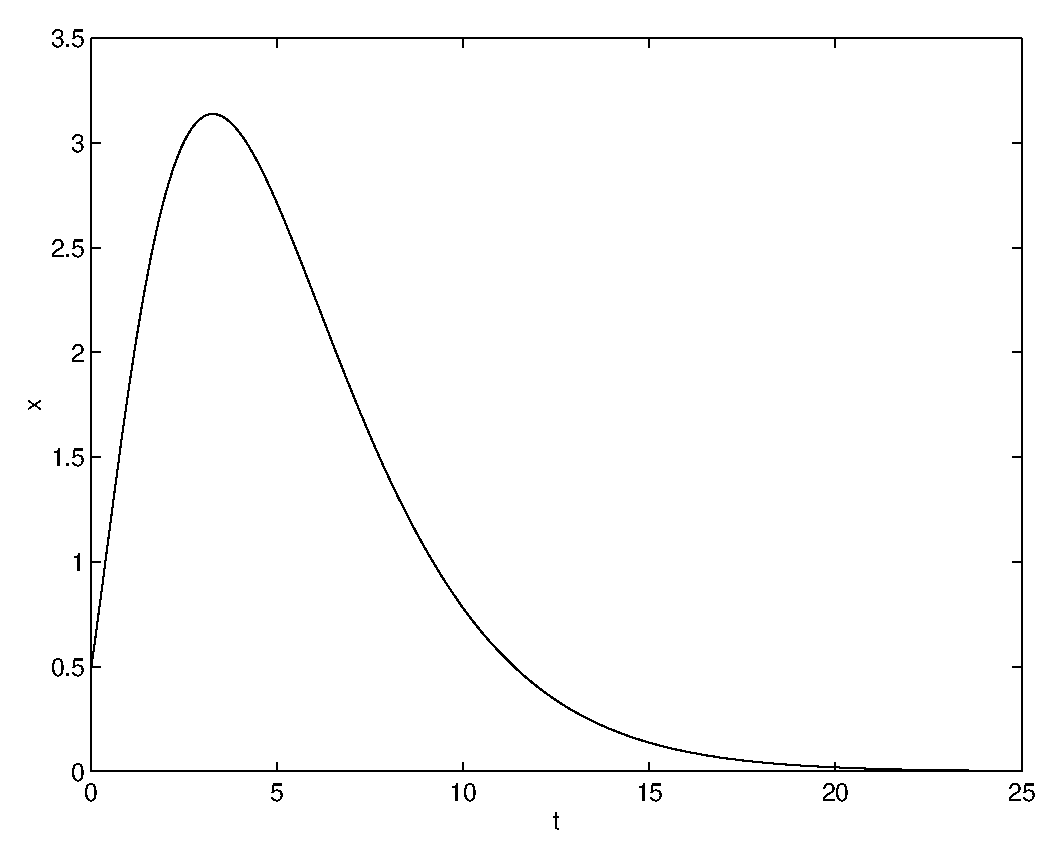
\psfig{file=figures/jordan.eps,width=3.5in}}
     \caption{First component $x_1(t)$ of solution to
	Jordan block equation for $k=3$ when $X(0)=(0.5,1.5,2)$.}
     \label{F:Jordan}
\end{figure}

\subsection*{Complex Eigenvalues}
\index{Jordan block}\index{Jordan block!with complex eigenvalue}

If $A$ is the Jordan block corresponding to a simple complex eigenvalue
$\lambda=\sigma+i\tau$, then \Ref{eq:linsys} is the two dimensional system 
\[
\frac{dX}{dt}=\mattwo{\sigma}{-\tau}{\tau}{\sigma} X
\]
whose solutions have the form 
\[
X(t)=e^{\sigma t}\mattwo{\cos(\tau t)}{-\sin(\tau t)} 
{\sin(\tau t)}{\cos(\tau t)} X_0.
\]

The general Jordan block corresponding to a multiplicity $k$ complex
eigenvalue $\sigma+i\tau$ has the form 
\begin{equation} \label{e:JM}
J + M
\end{equation}
where $J$ is a block diagonal\index{matrix!block diagonal} 
$2k\times 2k$ matrix with $k$ identical $2\times 2$ matrices 
\[
\mattwo{\sigma}{-\tau}{\tau}{\sigma}
\]
on the diagonal and $M$ is a $2k\times 2k$ block form matrix 
whose nonzero blocks have $I_2$ on the superdiagonal.

Since $J$ and $M$ commute, Proposition~\ref{P:expAB} of 
Chapter~\ref{Chap:Planar} implies that
\[
e^{t(J+M)} = e^{tJ} e^{tM}.
\]
As in the case of real eigenvalues $M^k=0$.  Now since $tJ$ is block 
diagonal, we can use Lemma~\ref{T:blocks} to determine that $e^{tJ}$ 
is also block diagonal with blocks 
\[
e^{\sigma t}\mattwo{\cos(\tau t)}{-\sin(\tau t)}{\sin(\tau t)}{\cos(\tau t)}.
\]
Putting these two observations together allows us to solve explicitly 
ODE systems whose coefficient matrix\index{matrix!coefficient}
is a single Jordan block\index{Jordan block} with complex eigenvalues.



\subsubsection*{An Example of a Complex Eigenvalue Jordan Block Equation}

Find the solution to the differential equation 
\[
\frac{dX}{dt} = \left(\begin{array}{rr|rr|rr} 
 2 & 1 & 1 & 0 & 0 & 0\\
-1 & 2 & 0 & 1 & 0 & 0 \\  
 \hline
 0 & 0 & 2 & 1 & 1 & 0 \\
 0 & 0 &-1 & 2 & 0 & 1 \\
\hline
 0 & 0 & 0 & 0 & 2 & 1\\
 0 & 0 & 0 & 0 &-1 & 2  \end{array}\right) X
\]
with initial condition
\[
X_0 = (1, 3, -2, 0, 0, 4).
\]

Using the notation of \Ref{e:JM} we have
\[
J = \left(\begin{array}{rr|rr|rr} 
 2 & 1 & 0 & 0 & 0 & 0\\
-1 & 2 & 0 & 0 & 0 & 0 \\  
 \hline
 0 & 0 & 2 & 1 & 0 & 0 \\
 0 & 0 &-1 & 2 & 0 & 0 \\
\hline
 0 & 0 & 0 & 0 & 2 & 1\\
 0 & 0 & 0 & 0 &-1 & 2  \end{array}\right) 
\AND 
M = \left(\begin{array}{rr|rr|rr} 
 0 & 0 & 1 & 0 & 0 & 0\\
0 & 0 & 0 & 1 & 0 & 0 \\  
 \hline
 0 & 0 & 0 & 0 & 1 & 0 \\
 0 & 0 & 0 & 0 & 0 & 1 \\
\hline
 0 & 0 & 0 & 0 & 0 & 0\\
 0 & 0 & 0 & 0 & 0 & 0  \end{array}\right).
\]
It follows that 
\begin{eqnarray*}
X(t) & = & e^{tJ}e^{tM}X_0 \\
 & = & e^{2t}\left(\begin{array}{rr|rr|rr} 
 \cos t & -\sin t & 0 & 0 & 0 & 0\\
\sin t & \cos t & 0 & 0 & 0 & 0 \\  
 \hline
 0 & 0 & \cos t & -\sin t & 0 & 0 \\
 0 & 0 & \sin t & \cos t & 0 & 0 \\
\hline
 0 & 0 & 0 & 0 & \cos t & -\sin t\\
 0 & 0 & 0 & 0 & \sin t & \cos t  \end{array}\right) 
\left(\begin{array}{rr|rr|rr} 
 1 & 0 & t & 0 & \half t^2 & 0\\
0 & 1 & 0 & t & 0 & \half t^2 \\  
 \hline
 0 & 0 & 1 & 0 & t & 0 \\
 0 & 0 & 0 & 1 & 0 & t \\
\hline
 0 & 0 & 0 & 0 & 1 & 0\\
 0 & 0 & 0 & 0 & 0 & 1  \end{array}\right) X_0 \\
 & = & e^{2t}\left(\begin{array}{rr|rr|rr} 
 \cos t & -\sin t & t\cos t & -t\sin t & \half t^2\cos t & -\half t^2\sin t\\
\sin t & \cos t & t\sin t & t\cos t & \half t^2\sin t & \half t^2\cos t \\  
 \hline
 0 & 0 & \cos t & -\sin t & t\cos t & -t\sin t \\
 0 & 0 & \sin t & \cos t & t\sin t & t\cos t \\
\hline
 0 & 0 & 0 & 0 & \cos t & -\sin t\\
 0 & 0 & 0 & 0 & \sin t & \cos t  \end{array}\right)
\left(\begin{array}{r} 1 \\ 3 \\ \hline -2 \\  0 \\ \hline 0 \\ 4
\end{array}\right).
\end{eqnarray*}
Finally,
\[
X(t) = e^{2t}\left(\begin{array}{c}
\cos t - 3\sin t -2t\cos t - 2t^2\sin t \\
\sin t + 3\cos t -2t\sin t + 2t^2\cos t \\
-2\cos t - 4t\sin t \\
-2\sin t + 4t\cos t \\
-4\sin t \\ 4\cos t \end{array}\right).
\]
Moreover, this example is typical of all such Jordan block equations. 

\subsection*{Solutions When Matrices are Not in Jordan Normal Form} 

Let $A$ and $B=S\inv AS$ be similar $n\times n$ matrices.  Recall 
Lemma~\ref{L:simsoln} of Chapter~\ref{Chap:Planar} which states that 
$X(t)=SY(t)$ is a solution to $\dot{X}=AX$ if and only if $Y(t)$ is a 
solution to
\begin{equation} \label{E:JNFDE}
\frac{dY}{dt} = BY.
\end{equation}

Suppose that $B$ is in Jordan normal form; then we know how to solve 
\Ref{E:JNFDE} using matrix exponentials and can then solve the original
equation $\dot{X}=AX$ in principle by multiplying $Y(t)$ by $S$.  This 
approach is clean in theory, but messy in practice.  

As an example, consider the differential equation $\dot{X}=AX$ where
\begin{equation*}
A = \left(\begin{array}{rrrr} 12 & 4 & 3 & 6 \\ 5 & 22 & 6 & -6\\
-34 & -69 & -22 & 7\\ -5 & 16 & 3 & -10 \end{array}\right),
\end{equation*}
with initial condition $X_0=(1,-1,0,1)^t$.  Use {\tt eig(A)} in \Matlab to 
verify that the eigenvalues of $A$ are $-1,-1,2,2$.  Since the nullities of 
$A+I_n$ and $A-2I_n$ both equal $1$, it follows that both double eigenvalues
have nontrivial Jordan blocks, and
\[
B = \mattwoc{\mattwo{-1}{1}{0}{-1}}{0}{0}{\mattwo{2}{1}{0}{2}}
\]
is the Jordan normal form of $A$.  As noted previously, we can solve 
\Ref{E:JNFDE} using matrix exponentials, obtaining
\[
Y(t) =
\mattwoc{e^{-t}\mattwo{1}{t}{0}{1}}{0}{0}{e^{2t}\mattwo{1}{t}{0}{1}}Y_0.
\]
To find a formula for $X(t)$ we need to find the matrix $S$ such that 
$B=S\inv AS$.  Then $X(t)=SY(t)$ where $Y_0=S\inv X_0$.  Using \Matlab we
can find vectors 
\begin{eqnarray*}
v_2 & \in & \nulls((A+I_n)^2)\setmin\nulls(A+I_n) \\
v_4 & \in & \nulls((A-2I_n)^2)\setmin\nulls(A-2I_n)
\end{eqnarray*}
Then set $v_1=(A+I_n)v_2$, $v_3=(A-2I_n)v_4$ and $S=(v_1|v_2|v_3|v_4)$. 
Indeed, 
\begin{verbatim}
S =
   -0.3580   -0.1181    0.2039   -0.0775
    0.3580   -0.2399    0.1019   -0.2936
   -0.3580    0.9559   -0.6116    0.9459
    0.7160   -0.1218   -0.1019   -0.1142
\end{verbatim}
and 
\begin{verbatim}
Y0 =
    5.5285
  -16.7608
   16.0879
   29.4307
\end{verbatim}
So 
\begin{equation}  \label{E:solvedebf}
X(t) = S\mattwoc{e^{-t}\mattwo{1}{t}{0}{1}}{0}{0}{e^{2t}\mattwo{1}{t}{0}{1}}
\left(\begin{array}{r} 5.5285 \\  -16.7608 \\ 16.0879 \\ 29.4307\end{array}
\right).
\end{equation}

\subsubsection*{The General Functional Form of Solutions}

The previous calculations suggest how to prove the following lemma.

\begin{lemma}  \label{R:pdeg}
Components of solutions to the system of differential equations $\dot{X}=AX$ 
where $A$ is an $n\times n$ matrix are linear combinations of the functions 
$t^je^{\lambda t}$ where $\lambda$ is a real eigenvalue of $A$ and 
$t^je^{\sigma t}\cos(\tau t)$ and $t^je^{\sigma t}\sin(\tau t)$ where
$\sigma\pm i\tau$ is a complex eigenvalue of $A$.   The exponent $j\leq k$, 
where $k$ is the size of the largest Jordan block associated to the given
eigenvalue. 
\end{lemma}

\proof  Formula \Ref{e:expsoln} verifies this statement when $A$ is in Jordan 
normal form with real eigenvalues.  A similar formula holds with $J$ and $M$ 
when $A$ has complex eigenvalues.  Solutions to the general matrix equation 
are just linear combinations of solutions to the corresponding Jordan normal 
form equations.  Indeed, as noted in the discussion leading to \Ref{E:JNFDE}, 
solutions to the general system equation are obtained from the Jordan normal 
form equations by multiplying these special solutions by the constant matrix
$S$.  This multiplication does not alter the statement that the coordinate
functions are linear combinations of the given functions.  \qed

In Section~\ref{S:SEOC} we discuss alternative methods for finding solutions 
to systems of constant coefficient linear differential equations.  All of
these methods require some effort to carry out by hand.


\EXER

\TEXER

\begin{exercise} \label{c11.1.1}
Find the solution to the system
\begin{eqnarray*}
\dot{x}_1 & = & 2x_1+x_2 \\
\dot{x}_2 & = & 2x_2 \\
\dot{x}_3 & = & x_3-x_4 \\
\dot{x}_4 & = & x_3+x_4
\end{eqnarray*}
satisfying $X_0=(-1,1,2,-3)^t$.
\end{exercise}

\begin{exercise} \label{c11.1.2}
Find the solution to the system
\begin{eqnarray*}
\dot{x}_1 & = & -2x_1+x_2+x_3 \\
\dot{x}_2 & = & -x_1-2x_2+x_4 \\
\dot{x}_3 & = & -2x_3+x_4 \\
\dot{x}_4 & = & -x_3-2x_4
\end{eqnarray*}
satisfying $X_0=(1,2,-1,-3)^t$.
\end{exercise}

\begin{exercise} \label{c11.1.3}
Let $X(t)$ be the solution to 
\[
\frac{dX}{dt} = \left(\begin{array}{rrr} 
-\half & 1 & 0 \\ 0 & -\half & 1\\ 0 & 0 & -\half
\end{array}\right)X
\]
satisfying $X_0=(0,1,1)^t$. Show that $X(2)$ is further from the 
origin than $X(0)$.
\end{exercise}

\begin{exercise} \label{c11.1.3A}
Consider the differential equation $\dot{X}=JX$ where $J$ is the single Jordan 
block $2\times 2$ matrix with double eigenvalue $0$.  Show that most 
solutions are unbounded in both forward and backward time.
\end{exercise}


\begin{exercise} \label{c11.1.3B}
Consider the differential equation $\dot{X}=JX$ where $J$ is the single Jordan 
block $4\times 4$ matrix with double eigenvalues $i$ and $-i$.  Show that most 
solutions spiral away from the origin in both forward and backward time.
\end{exercise} 

\begin{exercise} \label{c11.1.3C}
Find $e^J$ where 
\[
J = \left(\begin{array}{rrrr} 
1 & -2 & 1 &  0 \\ 
2 &  1 & 0 &  1 \\
0 &  0 & 1 & -2 \\
0 &  0 & 2 &  1
\end{array}\right).
\]
\end{exercise}

\begin{exercise} \label{c11.1.7}
Find $e^{tJ}$ where 
\[
J = \left(\begin{array}{rrrrr} 
-1 &  1 &  0 &  0 & 0 \\ 
 0 & -1 &  1 &  0 & 0 \\
 0 &  0 & -1 &  0 & 0 \\
 0 &  0 &  0 &  2 & 1 \\
 0 &  0 &  0 &  0 & 2
\end{array}\right).
\]
\end{exercise}

\CEXER

\begin{exercise} \label{c11.1.4}
Use calculus to compute the maximum value of the function $x_1(t)$ 
defined in \Ref{E:x1examp} and graphed in Figure~\ref{F:Jordan}.
\end{exercise}

\noindent In Exercises~\ref{c11.1.5A} -- \ref{c11.1.5B} solve the initial 
value problem $\dot{X}=AX$ for the given matrix $A$ and initial vector
$X_0$ in the form of \Ref{E:solvedebf} by converting $A$ to Jordan normal
form.
\begin{exercise} \label{c11.1.5A}
\begin{equation*}
A=\left(\begin{array}{rrr}  
    -3  &  -7 &   -2\\
    11  &  19  &   5\\
   -32  & -51 &  -13 \end{array} \right) \AND X_0=(1,0,-1)^t.
\end{equation*}
\end{exercise}
\begin{exercise} \label{c11.1.5B}
\begin{equation*}
A=\left(\begin{array}{rrrr}  
  103 &  138 &  124 &  -215 \\
  -67 &  -85 &  -68 &   142 \\
   22 &   27 &   20 &   -47 \\
   19 &   27 &   27 &   -39 \end{array} \right) \AND X_0=(1,2,0,3)^t.
\end{equation*}
\end{exercise}

In Exercises~\ref{c11.1.6A} -- \ref{c11.1.6B}, components of solutions to 
differential equation $\dot{X}=AX$ are linear combinations of functions of 
the form $t^je^{\lambda t}$ when $\lambda$ is a real eigenvalue of $A$ and 
$t^je^{\sigma t}\cos(\tau t)$ and $t^je^{\sigma t}\sin(\tau t)$ when
$\lambda=\sigma\pm i\tau$ is a complex eigenvalue of $A$.  Determine the
precise values of $j$ and $\lambda$ for each of the given matrices.  Do not
attempt to write down the closed form solutions to these systems of
differential equations.
\begin{exercise} \label{c11.1.6A}
\begin{equation*}
A=\left(\begin{array}{rrrr}  
   -3 &  77 & -124 & -225 \\
   10 &  -1 &   69 &  105 \\
  -26 & -47 & -112 & -148 \\
   18 &  24 &   89 &  124 \end{array} \right).
\end{equation*}
\end{exercise}
\begin{exercise} \label{c11.1.6B}
\begin{equation*}
A=\left(\begin{array}{rrrrrr}  
   29 &  27 &  -4 &  -7 &  -3 & -20 \\
  -26 & -23 &   5 &   9 &   3 &  23 \\
   12 &  26 &  -4 &  32 &   7 & -24 \\
   12 &  12 &  -3 &  -1 &  -1 & -13 \\
   -8 & -10 &   4 &  -3 &   1 &  16 \\
   -4 &  -8 &   2 &  -9 &  -2 &  10  \end{array} \right).
\end{equation*}
\end{exercise}



 
\section{Qualitative Theory Near Equilibria}
\label{S:QT}


In this section we discuss asymptotic stability and hyperbolicity for 
linear systems of differential equations.  We show, in general, that 
each linear constant coefficient system divides coordinates into three
groups: stable, center, and unstable.   Then, in analogy with the 
planar case, we discuss how solutions to nonlinear autonomous systems 
look very much like solutions to linear differential equations, at least
in a neighborhood of a hyperbolic equilibrium.


\subsection*{Asymptotic Stability}
\index{stability!asymptotic}


Consider the linear system of ODEs $\dot{X}=AX$.  In the case $n=2$ we showed 
that the origin is an asymptotically stable equilibrium precisely when the 
eigenvalues of $A$ have negative real part.  In this subsection we show that the 
same result holds for general $n$. 
\begin{Def}  \label{D:linstab}
The origin is a {\em linearly stable\/} equilibrium for the system 
of differential equations $\dot{X}=AX$ if the $n$ eigenvalues of $A$ 
all have negative real part.  
\end{Def}\index{stability!linear}
Using this definition we have:
\begin{thm}  \label{T:linstab}
The origin is an asymptotically stable equilibrium for the system of 
differential equations $\dot{X}=AX$ if and only if the origin is linearly stable.
\end{thm}

\proof The proof of this theorem follows directly from Lemma~\ref{R:pdeg}.
Each coordinate function of each solution of $\dot{X}=AX$ is a linear 
combination of functions of the form $t^je^{\lambda t}$ where $\lambda$ is 
a real eigenvalue of $A$ and $t^je^{\sigma t}\cos(\tau t)$ and 
$t^je^{\sigma t}\sin(\tau t)$ where $\lambda=\sigma\pm i\tau$ is a complex
eigenvalue of $A$.  Observe that if $\lambda < 0$, then
\[
\lim_{t\to\infty}t^ke^{\lambda t} = 0,
\]
since exponentials decay\index{exponential!decay} to zero faster than 
polynomials grow to infinity.  A similar argument holds when the multiple 
eigenvalue is complex since 
\[
\lim_{t\to\infty}t^ke^{\sigma t}\cos(\tau t) = 0 = 
\lim_{t\to\infty}t^ke^{\sigma t}\sin(\tau t),
\]
when $\sigma < 0$.  \qed

\subsection*{Stable, Unstable and Center Coordinates}

Recall from Chapter~\ref{Chap:PlanarQ} (Theorem~\ref{T:matrixcoord}) that 
two matrices are similar 
precisely when there is a linear change of 
coordinates\index{change of coordinates} that transforms
one matrix into the other.  Thus, when we assume that a matrix $A$ is in 
Jordan normal form\index{Jordan normal form} in the system of differential 
equations $\dot{X}=AX$, 
we are just assuming that we have made a preliminary change of coordinates
to put that matrix in normal form. 

We can always group the eigenvalues of a matrix into three classes: those 
that have negative real part\index{eigenvalue!with negative real part}, 
those that have positive real part\index{eigenvalue!with positive real part}, 
and those that have zero real part\index{eigenvalue!with zero real part}; and 
we can always arrange the Jordan normal form so 
that 
\begin{itemize}
\item[(i)] blocks corresponding to eigenvalues with negative real part come first,
\item[(ii)] blocks corresponding to eigenvalues with positive real part come 
next, and
\item[(iii)] blocks corresponding to eigenvalues with zero real part come last.
\end{itemize}
As a consequence of this discussion we have proved:
\begin{prop}  \label{P:SUC}
Every $n\times n$ matrix $B$ is similar\index{similar} to a 
block diagonal $n\times n$ matrix\index{matrix!block diagonal}
\begin{equation} \label{e:SUC}
A = \left(\begin{array}{ccc} S & 0 & 0 \\ 0 & U & 0\\ 0 & 0 & C \end{array}
\right),
\end{equation}
where
\begin{itemize}
\item[(a)]	$S$ is a Jordan normal form\index{Jordan normal form}
$k_s\times k_s$ matrix all of whose eigenvalues have negative real part;
\item[(b)]	$U$ is a Jordan normal form $k_u\times k_u$ matrix all
of whose eigenvalues have positive real part; and
\item[(c)]	$C$ is a Jordan normal form $k_c\times k_c$ matrix all
of whose eigenvalues have zero real part;
\end{itemize}
and $k_s+k_u+k_c=n$.
\end{prop}

Using Proposition~\ref{P:SUC}, we can give a qualitative description of 
every constant coefficient linear system of differential equations.
\begin{thm}  \label{T:SUC}
Let $A$ be a Jordan normal form matrix in the block diagonal form \Ref{e:SUC}.
Let $X=(x,y,z)\in\R^n$ where $x\in\R^{k_s}$, $y\in\R^{k_u}$ and $z\in\R^{k_c}$.
Then every solution to the differential equation $\dot{X}=AX$ has the form
\[
X(t) = (x(t), y(t),z(t)),
\]
where
\begin{itemize}
\item[(a)]  $x(t)$ decays to zero exponentially fast in 
	forward time and grows to 
	infinity exponentially fast in backward time;
\item[(b)]  $y(t)$ grows to infinity exponentially fast in forward time and 
	decays to zero exponentially fast in backward time; and
\item[(c)]  $z(t)$ can be either bounded or grow or decay. 
\end{itemize}
Moreover, if the Jordan blocks\index{Jordan block} of $C$ are all trivial
(that is, $1\times 1$ zero blocks or $2\times 2$ blocks with complex
conjugate purely imaginary eigenvalues), then $z(t)$ will remain bounded in 
both forward and backward time. 
\end{thm}

\proof  The block diagonal form of $A$ decouples the differential equation 
into three subsystems:
\begin{eqnarray*}
\dot{x} & = & Sx \\
\dot{y} & = & Uy \\
\dot{z} & = & Cz.
\end{eqnarray*}  
Since the eigenvalues of $S$ all have negative real part, Theorem~\ref{T:linstab} proves (a).  Since the eigenvalues of $U$ all have 
positive real part, we can run time backwards and obtain the differential 
equation $\dot{y}=-Uy$, where all of the eigenvalues of $-U$ have negative 
real part.  Again, we can use Theorem~\ref{T:linstab} to prove (b).  There 
is nothing to prove in part (c).  However, to prove the last statement, observe
that if the Jordan blocks in $C$ are trivial, then the blocks are either
$1\times 1$ zero blocks or $2\times 2$ blocks $\mattwo{0}{-\tau}{\tau}{0}$.
Solutions to the subblock equations are either equilibria (in the case of a
$1\times 1$ block) or circles (in the case of the $2\times 2$ block).  The
result follows, since the superposition of bounded solutions is bounded. \qed

\begin{Def}
The $x$ coordinates in Theorem~\ref{T:SUC} are the {\em stable\/} coordinates,
the $y$ coordinates are the {\em unstable\/} coordinates, and the $z$ 
coordinates are the {\em center\/} coordinates.
\end{Def}\index{coordinates!stable} \index{coordinates!unstable}
\index{coordinates!center}

Theorem~\ref{T:SUC} implies that for each linear constant coefficient system
of $n$ equations, we can group coordinates of $\R^n$ into stable, unstable,
and center coordinates for that differential equation.  Moreover, we just 
need to know the eigenvalues of the coefficient matrix to make this grouping.


\subsection*{Linearizations near Hyperbolic Equilibria}

Consider the autonomous\index{autonomous} system of differential equations 
\begin{equation} \label{e:eqnn}
\frac{dX}{dt} = f(X),
\end{equation}
where $X\in\R^n$ and $f:\R^n\to\R^n$.  We restate here for higher dimensional 
systems of 
differential equations some of the ideas and terminology that we introduced
previously for planar systems.  The point $X_0\in\R^n$ is an equilibrium 
\index{equilibrium} or steady-state solution\index{steady-state solution} 
if $f(X_0)=0$.  As we have seen, 
$X_0=0$ is an equilibrium of any linear system where $f(X)=AX$ for some 
$n\times n$ matrix $A$. 

Suppose that $X_0$ is an equilibrium for \Ref{e:eqnn}.  Let 
\[
f(X) = (f_1(X),\ldots,f_n(X))
\]
define the coordinate functions of $f$ as a function of $X=(x_1,\ldots,x_n)$.
Recall that the {\em Jacobian matrix\/}\index{matrix!Jacobian}
at $X_0$ is the $n\times n$ matrix of partial 
derivatives of $f$ and is denoted by $(df)_{X_0}$. \index{linearization} 
\index{matrix!Jacobian}  More precisely, 
\arraystart
\[
(df)_{X_0} = \left(\begin{array}{ccc}
\dps\frac{\partial f_1}{\partial x_1}(X_0) & \cdots & 
\dps\frac{\partial f_1}{\partial x_n}(X_0) \\ \vdots &  & \vdots \\
\dps\frac{\partial f_n}{\partial x_1}(X_0) & \cdots & 
\dps\frac{\partial f_n}{\partial x_n}(X_0) \end{array}\right).
\]
\arrayfinish
An equilibrium $X_0$ of \Ref{e:eqnn} is {\em hyperbolic\/} if the $n$
eigenvalues of $(df)_{X_0}$ all have nonzero real part. We now state 
the analog of Theorem~\ref{T:linearization} of Chapter~\ref{C:NPS}.
\index{hyperbolic}\index{equilibrium!hyperbolic}

\begin{thm}  \label{T:nlinearization}
Suppose that the system of differential equations \Ref{e:eqnn} has a 
hyperbolic equilibrium at $X_0$.  Then, on a sufficiently small neighborhood 
of $X_0$, the phase space for \Ref{e:eqnn} is the {\em same\/} as the phase 
space of the system of linear differential equations
\begin{equation}  \label{e:nlinearizedeqn}
\frac{dX}{dt} = (df)_{X_0}X.
\end{equation}
\end{thm} 

As before, it is difficult to define precisely what we mean by the word
{\em same\/}. Roughly speaking, {\em same\/} means that near $X_0$ there 
is a nonlinear change of coordinates\index{change of coordinates!nonlinear}
that transforms the nonlinear equation into the linear one.

\subsubsection*{Asymptotically Stable Equilibria in Nonlinear Systems}
\index{equilibrium!asymptotically stable}

We illustrate this theorem and consider the linear system 
$\dot{X}=AX$ where $A$ is given by
\begin{equation*}  \label{eq:fexam4}
A = 
\left(\begin{array}{rrrr}
   -0.1 &  0.1 & -0.2 &  0.1\\
   -0.8 & -0.5 &  1.9 &    0\\
    2.4 & -3.9 & -0.7 &  0.1\\
    0.3 &  0.1 & -0.2 & -0.3
\end{array}\right)
\end{equation*}
We can enter $A$ into \Matlab and compute the eigenvalues of $A$ by typing 
\begin{verbatim}
e12_2_4
eig(A)
\end{verbatim}\index{\computer!eig}
and we obtain
\begin{verbatim}
ans =
  -0.5725+ 2.8194i
  -0.5725- 2.8194i
  -0.0550         
  -0.4000         
\end{verbatim}
In particular, all eigenvalues of $A$ have negative real parts, and 
Theorem~\ref{T:linstab} implies that the origin is an asymptotically 
stable equilibrium\index{equilibrium!asymptotically stable}.

Theorem~\ref{T:nlinearization} implies that the origin remains
asymptotically stable for any system of differential equations
\begin{equation} \label{e:fnonlin}
\dot{X} = AX + N(X),
\end{equation}
where $N(X)$ consists only of higher order terms.  For example, suppose
\begin{equation}  \label{E:fnonlin1}
N(X) = \left(\begin{array}{c} 2x_1^2-x_1x_2 \\ -x_4^3 \\  -x_3^2 \\ x_4x_1
\end{array} \right).
\end{equation}
Then the Jacobian matrix of the right hand side in \Ref{e:fnonlin} at $X_0 = 0$ 
is given by $A$ and Theorem~\ref{T:nlinearization} guarantees that solutions to 
the nonlinear equation \Ref{e:fnonlin} that have an initial condition near 
enough to the origin will tend towards the origin in forward time.  It would be 
nice to test the consequences of this theorem numerically, but until now we
have not discussed how to integrate solutions to differential equations in
more than two dimensions.  We will do this in Section~\ref{S:ode45HD} using a 
three dimensional equation. 

\subsubsection*{Saddles, Sources and Sinks in Higher Dimensions}

Suppose that one eigenvalue $\lambda$ of the $n\times n$ matrix $A$ has 
positive real part.  Then {\em almost all\/} solutions to the linear system 
$\dot{X}=AX$ tend to infinity in forward time.  This 
statement can be proved by appealing to Theorem~\ref{T:SUC}.    

It follows from Theorem~\ref{T:nlinearization} that if $X_0$ is an
equilibrium\index{equilibrium} and one eigenvalue of $(df)_{X_0}$ has positive 
real part, then almost all solutions near the equilibrium $X_0$ will leave 
small neighborhoods of that equilibrium in forward time.  Thus, in this case 
the equilibrium is not asymptotically stable.

Note that if $(df)_{X_0}$ has an eigenvalue with positive real part and an
eigenvalue with negative real part, then most solutions with initial
conditions near $X_0$ will leave small neighborhoods of $X_0$ in both forward
and backward times.  Such equilibria are called {\em saddles\/}.\index{saddle}

Equilibria are called {\em sources\/}\index{source} when all the eigenvalues 
of the corresponding Jacobian have positive real parts and 
{\em sinks\/}\index{sink} when all the eigenvalues of the corresponding 
Jacobian have negative real parts.



\EXER

\TEXER  

\noindent In Exercises~\ref{c14.2.1A} -- \ref{c14.2.1B} compute the Jacobian 
matrices of the given system of differential equations at the given point.
\begin{exercise} \label{c14.2.1A}
$\left\{\begin{array}{rcl} 
\dot{x} & = & -10 + 2x - z - 3x^2+y^2 \\
\dot{y} & = & x + y + 2xz \\
\dot{z} & = & -27 + z + 10xy - x^2  \end{array}\right.$ 
\AND $(x_0,y_0,z_0) = (2,-1,4)$.
\end{exercise}
\begin{exercise} \label{c14.2.1B}
$\left\{\begin{array}{rcl} 
\dot{x} & = & 2 + 2z + x^2 - z^3 \\
\dot{y} & = & x + xyz \\
\dot{z} & = & -10 + y + 10xy + x^3  \end{array}\right.$ 
\AND $(x_0,y_0,z_0) = (1,2,-2)$.
\end{exercise}

\begin{exercise} \label{c14.2.1C}
Verify that $(1,3,-2)$ is an equilibrium for the differential equation in 
Exercise~\ref{c14.2.1A}.  Is this equilibrium asymptotically stable or not?
\end{exercise}

\begin{exercise} \label{c14.2.1D}
Verify that $(1,1,-1)$ is an equilibrium for the differential equation in 
Exercise~\ref{c14.2.1B}.  Is this equilibrium asymptotically stable or not?
\end{exercise}

\begin{exercise} \label{c14.2.1E}
Consider the system of ODEs $\dot{X}=F(X)$ where
\[
F(x,y,z) = (x^2 - z, y^2 - z, 2x + y - 3).
\]
Find all equilibria of this system and determine the number of stable and 
unstable directions for each of these equilibria.
\end{exercise}

\begin{exercise} \label{c14.2.1F}
Consider the system of ODEs $\dot{X}=F(X)$ where
\[
F(x,y,z) = (x - 2y - x^2, y + z^2, -z - x^2).
\]
Find all equilibria of this system and determine the number of stable and 
unstable directions for each of these equilibria.
\end{exercise}

\CEXER

\noindent In Exercises~\ref{c11.2.1a} -- \ref{c11.2.1c} determine whether 
the origin is an asymptotically stable equilibrium for the system of 
differential equations $\dot{x}=Cx$.
\begin{exercise} \label{c11.2.1a}
\[
C=\mattwo{1}{-3}{2}{-5}.
\]
\end{exercise}
\begin{exercise} \label{c11.2.1b}
\begin{equation*}
C=\left(\begin{array}{rrr} 
94 & 174 & 132 \\ 
-37 & -68 & -53 \\
-16 & -29 & -24 \end{array}\right).
\end{equation*}
\end{exercise}
\begin{exercise} \label{c11.2.1c}
\begin{equation*}
C=\left(\begin{array}{rrrr} 
-0.28 & -0.04 & -0.22 & -0.42 \\ 
0.16 & -0.62 & 0.14 & 0.04 \\ 
0.06 & -0.12 & -0.06 & 0.14 \\ 
0.04 & -0.28 & 0.06 & -0.34 \end{array}\right).
\end{equation*}
\end{exercise}

\noindent In Exercises~\ref{c11.2.2a} -- \ref{c11.2.2c} determine the number
of stable, unstable, and center directions for the system of differential 
equations $\dot{x}=Cx$.
\begin{exercise} \label{c11.2.2a}
\begin{equation*}
C=\left(\begin{array}{rrrr}
     1  &   2   &  3   &  4 \\
     5  &   4   &  3   &  2\\
     9  &   8   &  7   &  6\\
     1  &   2    & 6   &  7
\end{array}\right).
\end{equation*}
\end{exercise}
\begin{exercise} \label{c11.2.2b}
\begin{equation*}
C=\left(\begin{array}{rrrrr}
     1   &  3  &   6   &  9   & 11 \\
    -2   &  4  &   6   & -8   & 0 \\
     1   &  3  &   5   &  7   & 9 \\
     0   &  2  &   5   &  8   &  0 \\
     1   &  4  &  -2   &  4   & 10
\end{array}\right).
\end{equation*}
\end{exercise}
\begin{exercise} \label{c11.2.2c}
\begin{equation*}
C=\left(\begin{array}{rrrrrr}
    1  &  3  &  5  & -11 &  20  &   5 \\
   -5  & -13 & -11 &  23 & -49  & -12 \\
   13  &  47 &  41 & -82 & 167  &  41 \\
    4  &  35 &  27 & -48 &  94  &  23 \\
    8  &  10 &   6 & -16 &  45  &  11 \\
  -30  &  -8 &  -2 &  28 &-110  & -27
\end{array}\right).
\end{equation*}
\end{exercise}





\section{MATLAB {\tt ode45} in One Dimension}  \label{S:ode45}

Previously, we have used {\sf dfield5}, {\sf pline}, and {\sf pplane5}
to compute solutions to one and two dimensional ordinary differential
equations numerically.  We now wish to compute solutions to higher dimensional
systems of ordinary differential equations and to do this we will use the 
\Matlab command {\tt ode45}.\index{\computer!ode45}  \Matlab provides the 
command {\tt ode45}, among others, for solving initial value problems, and we 
illustrate how this command works on several examples.  In this section we 
illustrate the command on a simple one dimensional example and in the next
section we will compute solutions to three and four dimensional systems.

\subsubsection*{A Simple One Dimensional Example}

Suppose that we want to compute numerically the solution of the initial value 
problem\index{initial value problem}
\arraystart
\begin{equation}   \label{eq:fexam}
\begin{array}{rcl}
\dps \frac{dx}{dt}(t) & = & x(t)+t \\
x(t_0) & = & x_0
\end{array}
\end{equation}
\arrayfinish
on the time interval $t\in [t_0,t_e]$.  Then the {\em data\/} of this 
problem are 
\begin{itemize}
\item the numbers $x_0,t_0$ and $t_e$, and 
\item the function $f(t,x)=x+t$.  
\end{itemize}
We know how to assign specific values for $t_0,x_0$ and $t_e$ in \Matlabp;
we will call these variables {\tt t0, x0} and {\tt te}.  Before proceeding, 
we need to understand how to make a function $f(t,x)$ available for 
computations in \Matlabp.

\subsection*{The Construction of m-files in MATLAB}\index{\computer!m-file}

Functions that are used by \Matlab are defined via 
{\em m-files}.  We now show how to construct m-files with two examples.

Suppose that we want the function $g:\R^2\to\R$, defined by
\begin{equation*}  \label{eq:gexam}
g(y,z) = yz^2 + \sin y,
\end{equation*}
to be available in \Matlabp.
Then we specify $g$ by writing a \Matlab m-file that contains the information 
defining this function.  The m-file {\tt gexam.m} that defines the function 
$g(y,z)$ in \Ref{eq:gexam} has two lines:
\begin{verbatim}
function g = gexam(y,z)
g = y*z^2 + sin(y);
\end{verbatim}\index{\computer!function}
The first line states that 
\begin{itemize}
\item this m-file contains a {\tt function} with the name {\tt gexam},
\item the input arguments are {\tt y} and {\tt z}, and
\item the output variable is {\tt g}.
\end{itemize}
The value of the function $g$ at the point ${\tt (y,z)}$ is given in the 
second line 
\begin{verbatim}
g = ... ;   
\end{verbatim}
Note that this line must end with a semicolon. 
\begin{quote}
{\bf Remark:} When \Matlab is used under Windows or on a PowerMac, then 
m-files
can be created using the {\sf New} entry in the {\sf File} menu.
On Unix based systems we must create the m-file using a separate
editor.  In any case make sure that the new m-file is stored in the directory
where \Matlab has been started.
\end{quote}
As an exercise, create the m-file {\tt gexam.m}.  The function $g$ is 
now available in \Matlabp; when we type {\tt gexam(1,2)}, 
we obtain the answer \verb+4.8415+, which is indeed $g(1,2)=4+\sin(1)$.

We store function m-files with the other {\sf laode} files using the prefix
{\tt f} (for function) followed by the equation number.  So the m-file 
{\tt gexam.m} is stored as {\tt f14\_3\_2.m}.  Indeed, compare the result of 
typing {\tt f14\_3\_2(1,2)} with {\tt gexam(1,2)}.

Both the input arguments and the output variable in an m-file can consist of 
vectors\index{vector}.  For instance, suppose that we want to define the function 
$h:\R^3\to\R^2$ where $u=(u_1,u_2,u_3)^t\in\R^3$ and  
\begin{equation*}
h(u) = \left(\begin{array}{c} u_1 u_2\\ u_2-u_1 u_3 \end{array}\right).
\end{equation*}
As a second exercise, write the m-file\index{\computer!m-file} {\tt hexam.m} 
as follows:
\begin{verbatim}
function h = hexam(u)
h = [u(1)*u(2), u(2)-u(1)*u(3)]';
\end{verbatim}
The command {\tt w = hexam([1,2,3])} gives the answer
\begin{verbatim}
w =
     2
    -1
\end{verbatim}
which is indeed $h(1,2,3)$.  This m-file has been stored as {\tt f14\_3\_3.m}.

\subsection*{The \Matlab Command {\tt ode45}}\index{\computer!ode45}

We now return to the initial value problem \Ref{eq:fexam}.
The function 
\begin{equation*}
f(t,x)=x+t
\end{equation*}
on the right hand side is available to \Matlab in the m-file 
{\tt f14\_3\_4.m}, which is stored with the other {\sf laode\/} files: 
\begin{verbatim}
function f = f14_3_4(t,x)
f = x + t;
\end{verbatim}

The \Matlab command 
\begin{center}
{\tt ode45('f14\_3\_4',[t0 te],x0)}
\end{center}\index{\computer!ode45} 
computes a numerical approximation to the solution to the initial value 
problem \Ref{eq:fexam} on the interval {\tt [t0,te]}.
For instance, we can use {\tt ode45} to solve the initial value problem
\begin{equation}  \label{eq:fexam1}
\begin{array}{rcl}
\dps \frac{dx}{dt} & = & x+t \\
x(1) & = & 2
\end{array}
\end{equation}
for $t\in[1,3]$. In this case, $t_0=1$, $t_e=3$, and $x_0=2$.  After 
typing the command
\begin{verbatim}
[t,x] = ode45('f14_3_4',[1 3],2);
\end{verbatim}
the approximate solution is stored in the vectors {\tt t} and {\tt x}.
The components of the vector {\tt t} are the values of $t$ for which the 
solution has been computed, and the components of the vector {\tt x} are 
the values of the solution $x$ at the values {\tt t}.  Indeed, typing 
{\tt t} and {\tt x} we see that both vectors have length $45$.   The
length of the vectors {\tt t} and {\tt x} is chosen by {\tt ode45} so
as to guarantee a certain accuracy in the solution.  We discuss this 
issue in greater detail below.

We can visualize the solution by plotting its time series\index{time series}:
\begin{verbatim}
plot(t,x)
xlabel('t')
ylabel('x')
\end{verbatim}\index{\computer!plot}
The result is shown in Figure~\ref{fig:ode45ex1}.  

\begin{figure}[htb]
   \centerline{%
   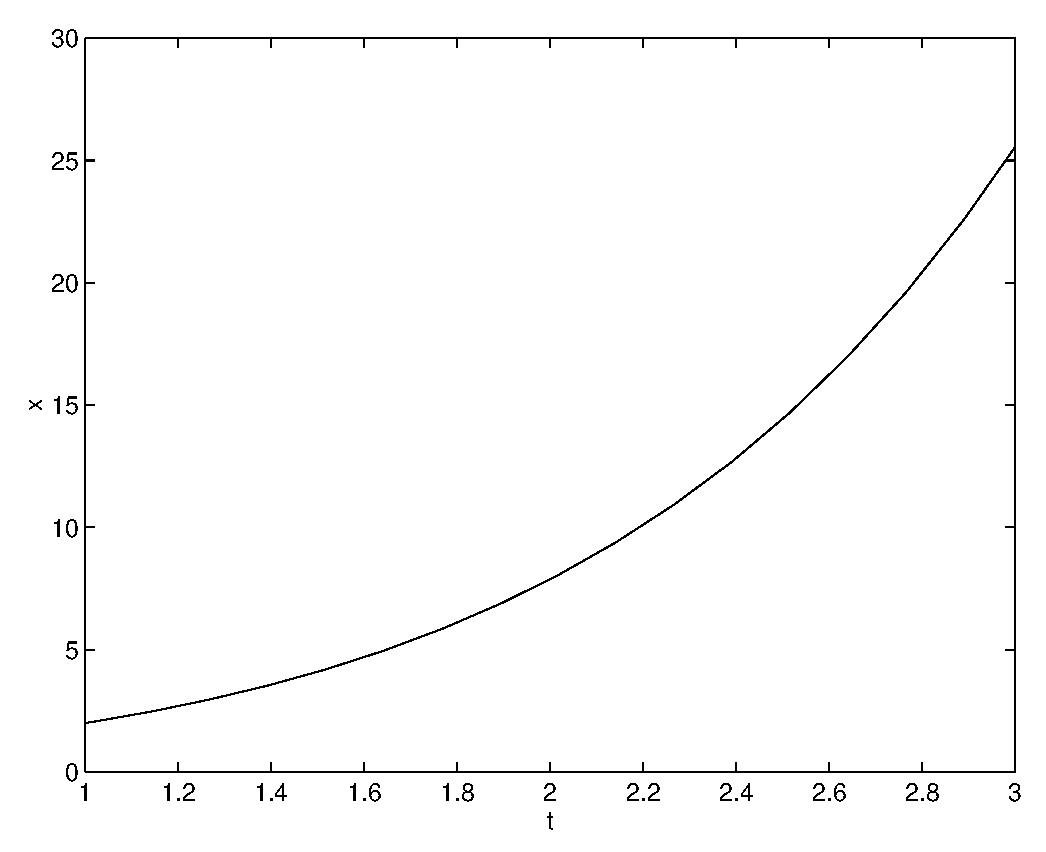
\psfig{file=figures/ode45ex1.eps,width=3.2in}}
   \caption{Approximation of the solution of
   \protect\Ref{eq:fexam1} obtained by {\tt ode45} in \protect\Matlabp.}
   \label{fig:ode45ex1}
\end{figure}

In fact, the initial value problem \Ref{eq:fexam1} has a simple closed form 
solution
\[
x(t) = 4e^{t-1}-t-1,
\]
which can be verified directly by differentiation.  The existence of this
closed form solution allows us to check the accuracy of the numerical
calculations made by {\tt ode45}.  Indeed, graphically we cannot distinguish 
the result obtained using {\tt ode45}\index{\computer!ode45} from the exact 
solution.  To verify this point, type
\begin{verbatim}
x_exact = 4*exp(t-1)-t-1;
hold on
plot(t,x_exact,'r')
\end{verbatim}
and observe that the graph of the exact solution, which is in red, exactly
covers the plot of the numerically computed solution.

\subsection*{Accuracy of {\tt ode45}}
\index{accuracy of {\tt ode45}}

We now discuss the error made by {\tt ode45} in more detail.
\index{\computer!ode45}
Using {\tt ode45} we obtained an approximation of the solution of
the initial value problem \Ref{eq:fexam1} at the times $t_k={\tt t(k)}$
for $k=1,2,\ldots,45$.  The exact solution at these points is
\[
x(t_k)=4e^{t_k-1}-t_k-1,
\]
and the {\tt ode45} approximation to the solution is $x_k={\tt x(k)}$.  The 
routine {\tt ode45} automatically computes the solution subject to satisfying 
two constraints: {\em absolute error} and {\em relative error\/}.

The {\em absolute error}\index{error!absolute} is just the absolute value of
the difference between the numerically computed solution and the exact
solution, that is,
\[
\epsilon_{abs}(k) = |x_k - x(t_k)|.
\]
We can visualize the absolute error by plotting $\epsilon_{abs}$ versus $t$, 
as follows:
\begin{verbatim}
err_abs = abs(x-x_exact);
plot(t,err_abs)
xlabel('t')
ylabel('absolute error')
\end{verbatim}
The \Matlab command {\tt abs(v)} generates a vector containing the absolute 
values of the components of the vector {\tt v}.  The result is presented in 
Figure~\ref{fig:ode45err0}.  Note that even though the absolute error 
oscillates, it is always less than $6\cdot10^{-6}$, which is why we could not 
distinguish the graph of the exact solution from the graph of the numerically 
computed solution given in Figure~\ref{fig:ode45ex1}.

\begin{figure}[htb]
   \centerline{%
   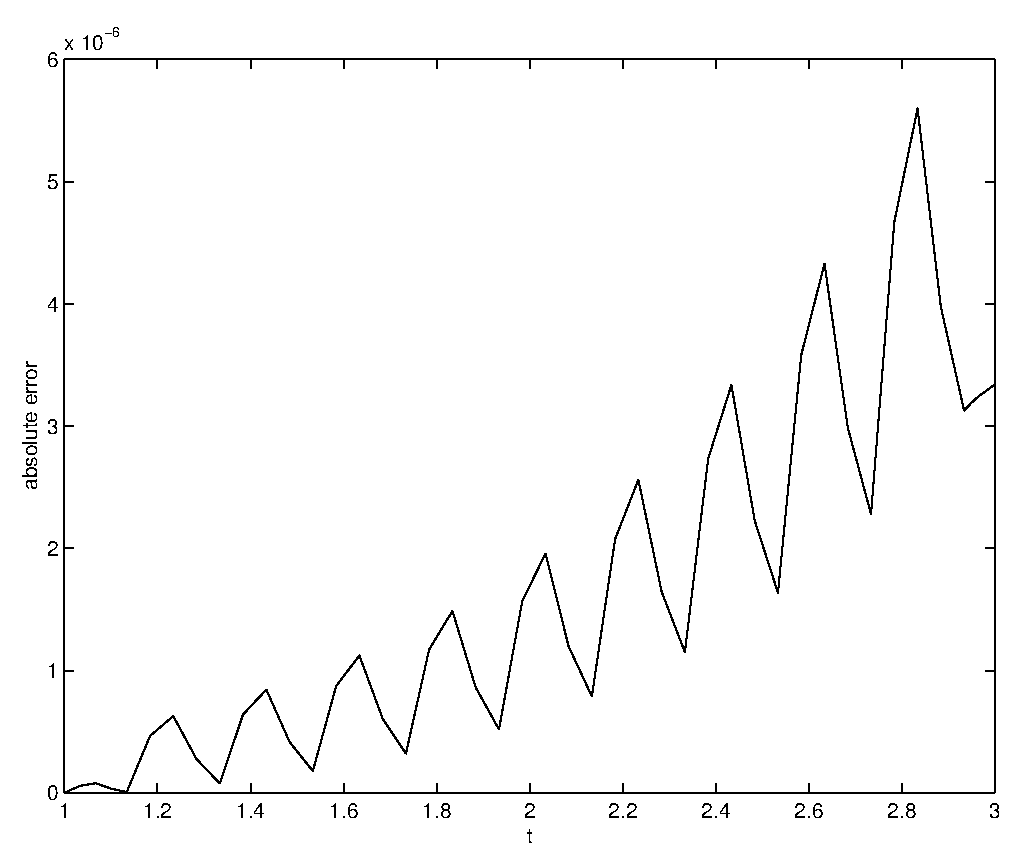
\psfig{file=figures/ode45err0.eps,width=3.2in}}
   \caption{Absolute error in the approximation of the solution of
   \protect\Ref{eq:fexam1} obtained by {\tt ode45} in \protect\Matlab with 
	default error bound {\tt 1e-6}.}
   \label{fig:ode45err0}
\end{figure}

Having an absolute error of $10^{-6}$ in a numerically computed solution might
seem quite good --- unless we happened to be computing a solution whose size 
is $10^{-7}$.  Then the numerical error would be ten times the size of the 
solution itself, which is a huge error.  For this reason, numerical analysts
like to use another measure for success.  

The {\em relative error\/}\index{error!relative} between 
the approximation and the exact solution is the absolute error normalized by 
the size of the exact solution, that is  
\[
\epsilon_{rel}(k) = \frac{\epsilon_{abs}(k)}{|x(t_k)|} 
= \frac{|x_k - x(t_k)|}{|x(t_k)|}.
\]
The numbers $\epsilon_{rel}(k)$ must be uniformly small in order to guarantee
a good numerical approximation to the actual solution.  Using the fact
that we have a formula for the exact solution, we can compute the numbers 
$\epsilon_{rel}$ and plot them in \Matlab by typing
\begin{verbatim}
err_rel = abs(x-x_exact)./abs(x_exact);
plot(t,err_rel)
xlabel('t')
ylabel('relative error')
\end{verbatim} 
The result is shown in Figure~\ref{fig:ode45err1}.  We see that the relative 
error oscillates, but is always smaller than $3\cdot 10^{-7}$.
\begin{figure}[htb]
   \centerline{%
   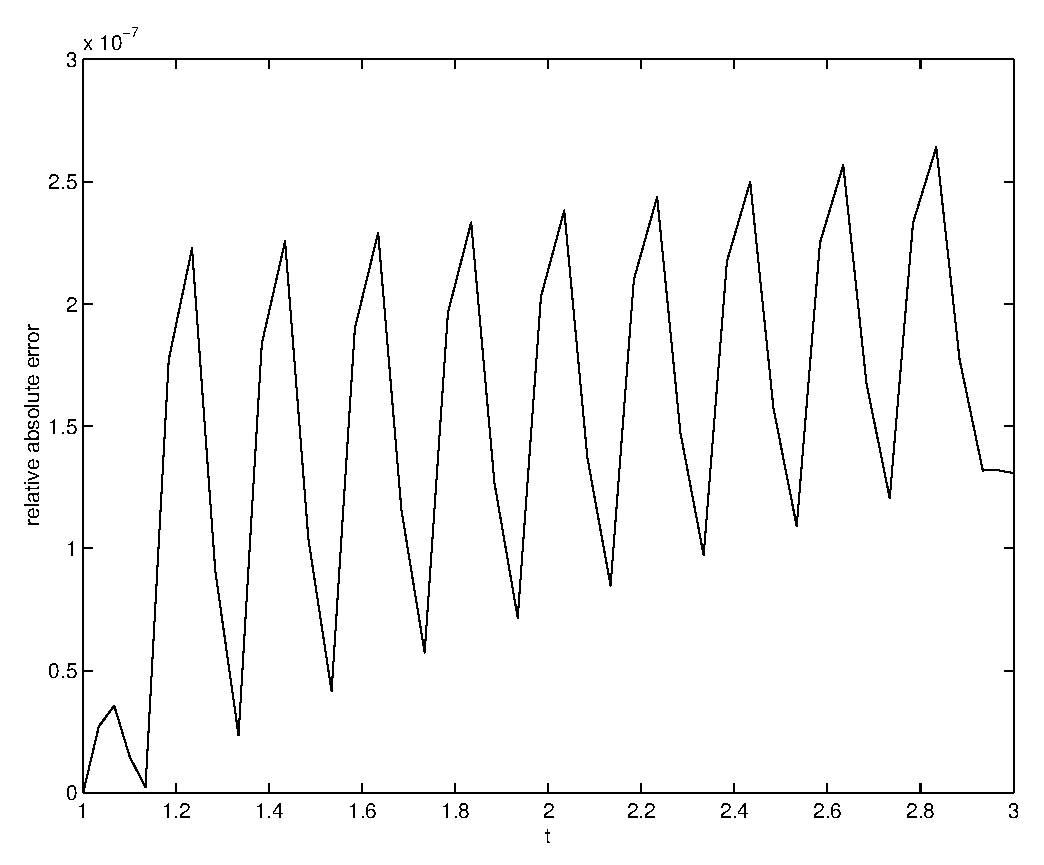
\psfig{file=figures/ode45err1.eps,width=3.2in}}
   \caption{Relative error in the approximation of the solution of
   \protect\Ref{eq:fexam1} obtained by {\tt ode45} in \protect\Matlab with 
	default error bound {\tt 1e-3}.}
   \label{fig:ode45err1}
\end{figure}

Default error bounds are preset in the command {\tt ode45}.  Unless otherwise
instructed {\tt ode45} {\em attempts\/} to find a numerical approximation 
whose absolute error is everywhere less than $10^{-6}$ and whose relative 
error is everywhere less than $10^{-3}$.  (There is a interesting mathematical
question concerning how these bounds are actually satisfied, since 
{\tt ode45} does not, in fact, know the exact solution.)  We can use 
{\tt ode45} to compute an approximation of the solution with an even smaller 
error.  To set this smaller error, we add an argument to the call of 
{\tt ode45} by typing 
\begin{verbatim}
options = odeset('RelTol',1e-8);
[t,x]=ode45('f14_3_4',[1 3],2,options);
\end{verbatim}
These instructions compute an approximation for which the relative error 
\index{error!relative} is smaller than $10^{-8}$.  
(Type {\tt odeset}\index{\computer!odeset} in \Matlab in order to see a 
complete list of options. Type {\tt options} to see a list of the currently
specified options.)  Hence, when we perform 
this calculation, we expect to obtain an even better result than before.  
Indeed, proceeding as above, we obtain the relative error shown 
in Figure~\ref{fig:ode45err2}.  In an attempt to guarantee the reduced error, 
{\tt ode45} generates 61 time steps during the computation.  

\begin{figure}[htb]
   \centerline{%
   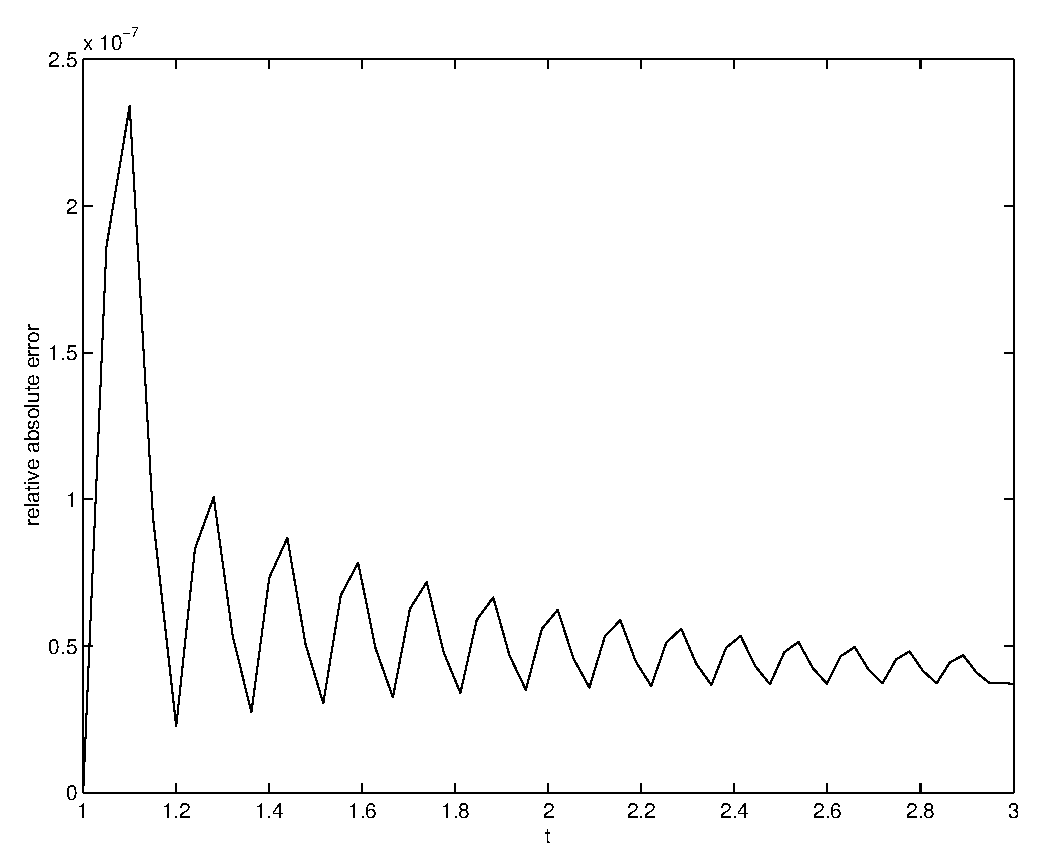
\psfig{file=figures/ode45err2.eps,width=3.2in}}
   \caption{Relative error in the approximation of the solution of
   \protect\Ref{eq:fexam1} obtained by {\tt ode45} in \protect\Matlab with 
	{\tt 1e-8} error bound.}
   \label{fig:ode45err2}
\end{figure}

\EXER

\CEXER

\noindent For each function specified in Exercises~\ref{c11.3.2a} -- 
\ref{c11.3.2f}, write an m-file that makes that function available in 
\Matlabp.
\begin{exercise} \label{c11.3.2a}
$f1:\R\to\R$ where $f1(t)=\sin(t) - t^3$.
\end{exercise}
\begin{exercise} \label{c11.3.2b}
$f2:\R^2\to\R$ where $f2(x,y)=x(1-y)$.
\end{exercise}
\begin{exercise} \label{c11.3.2c}
$f3:\R^2\to\R^2$ where  
$f3(x,y)=\left(\begin{array}{c} xy-1\\x+2y\end{array}\right)$.
\end{exercise}
\begin{exercise} \label{c11.3.2d}
$f4:\R^3\to\R$ where $f4(u)=u_1-u_2^2 + u_3$ and $u=(u_1,u_2,u_3)^t$.
\end{exercise}
\begin{exercise} \label{c11.3.2e}
$f5:\R^3\to\R^2$ where $f5(u)=\left(\begin{array}{c} u_1 -2u_3\\u_1 u_2 u_3\end{array}\right)$ and $u=(u_1,u_2,u_3)^t$.
\end{exercise}
\begin{exercise} \label{c11.3.2f}
$f6:\R^3\to\R^3$ where $f6(u)=\left(\begin{array}{c} u_3\\u_1 u_3\\ 
\sin u_2\end{array}\right)$ and $u=(u_1,u_2,u_3)^t$.
\end{exercise}

\begin{exercise} \label{c11.3.2A}
Verify that $x(t) = e^{\frac{1}{2}(t^2-4)}$ is a solution to the initial 
value problem
\[
\begin{array}{rcl}
\dot{x} & = & tx \\
x(2) & = & 1.
\end{array}
\]
Use {\tt ode45} to compute the solution to this initial value problem on the
interval $[2,3]$ to within an accuracy $10^{-6}$ and graphically compare this 
answer with the graph of the exact solution.  Find the values $x(2.5)$ and
$x(2.75)$.  {\bf Hint}: Set the exact times $t$ where the ODE solver 
evaluates time by the command {\tt tspan = 2:0.01:3;} and insert {\tt tspan}
instead of the interval {\tt [2,3]} in {\tt ode45}.  Use {\tt help ode45} in 
\Matlab for additional information. 
\end{exercise}

\begin{exercise}  \label{c11.3.2B}
Verify that $x(t) = e^{(1-\cos t)}$ is a solution to the initial value problem
\[
\begin{array}{rcl}
\dot{x} & = & x\sin t \\
x(0) & = & 1.
\end{array}
\]
Use {\tt ode45} to compute the solution to this initial value problem on the
interval $[0,15]$ to within an accuracy $10^{-4}$ and graphically compare 
this answer with the graph of the exact solution.  Find the values $x(2)$ 
and $x(3)$. 
\end{exercise}



\section{Higher Dimensional Systems Using {\tt ode45}}
\label{S:ode45HD}

In this section we discuss how to use {\tt ode45} to find solutions to linear
and nonlinear systems of differential equations in three dimensions, and how 
to plot the results of these calculations.  The same ideas will work in 
principle in any numbers of dimensions.  Specifically, we compute the solutions 
of a nonlinear system and its linearization at a hyperbolic equilibrium.  In 
this example we test numerically the conclusions of 
Theorem~\ref{T:nlinearization} on linearized stability for nonlinear systems.

 
\subsubsection*{A Three Dimensional Linear Example}

We now use {\tt ode45} to numerically compute solutions of the system
$\dot{X} = AX$ where 
\begin{equation}  \label{E:3dexample}
A = \left(\begin{array}{rrr}
  -0.25 & 3.00 & 0\\
   -3.00 & -0.25 &  0\\
   0 &  0 & -0.2
\end{array}\right).
\end{equation}
The function  
\begin{equation*}
f(X) = AX
\end{equation*}
that is on the right hand side of this linear system of differential 
equations is stored in the m-file {\tt f14\_4\_2.m}.  The following lines 
are included in that m-file.
\begin{verbatim}
function f = f14_4_2(t,x)
A = [ -0.25 3.0 0; -3 -0.25 0; 0 0 -0.2];
f = A*x;
\end{verbatim}
Observe that the first argument of the function {\tt f14\_4\_2} has to be 
$t$ even though this variable does not explicitly occur on the right hand 
side.  

The eigenvalues of $A$ are $-0.25\pm 3i$ and $-0.2$.  It follows that in the 
$x_1x_2$ plane solutions spiral into the origin and along the $x_3$ axis 
solutions decay exponentially to the origin.  By superpositon most solutions
will spiral around the $x_3$ axis while decaying into the origin.  We test 
this prediction using {\tt ode45}.

We approximate the solution starting in $X_0=(2,-1,-1)$ using
{\tt ode45} on the time interval $[0,100]$ by typing
\begin{verbatim}
[t,x] = ode45('f14_4_2',[0 100],[2,-1,-1]');
\end{verbatim}
Note that when using {\tt ode45},\index{\computer!ode45} the 
initial condition must be entered 
as a {\em column\/} vector.   (The reason is that this vector is an
input argument of the function {\tt f14\_4\_2} and in this function
this argument is multiplied by the matrix {\tt A}.)  When the computation 
is complete, 
the approximation of $(t,x_1(t),x_2(t),x_3(t))$ is stored in the column 
vector {\tt t} and in the three columns of the matrix {\tt x}.  Indeed, if 
we type {\tt size(t)} or {\tt size(x)}, then we see that {\tt t} is a 
vector of length $897$ and {\tt x} is a matrix with $897$ rows and $3$ 
columns.  

Next we consider how to graphically view the solutions.  As in one and
two dimensions, there are two possibilities.  First, we can visualize 
the three time series\index{time series} 
$(t,x_1(t))$, $(t,x_2(t))$ and $(t,x_3(t))$.  
This can be done by typing
\begin{verbatim}
subplot(3,1,1)
plot(t,x(:,1))
ylabel('x1')
subplot(3,1,2)
plot(t,x(:,2))
ylabel('x2')
subplot(3,1,3)
plot(t,x(:,3))
ylabel('x3')
xlabel('t')
\end{verbatim}
\index{\computer!subplot}\index{\computer!plot}
We then obtain the result shown in Figure~\ref{fig:flinear1}.  This figure 
shows the expected oscillation in the $x_1$ and $x_2$ coordinates and the 
exponential decay in the $x_3$ coordinate.
\begin{figure}[htb]
   \centerline{%
   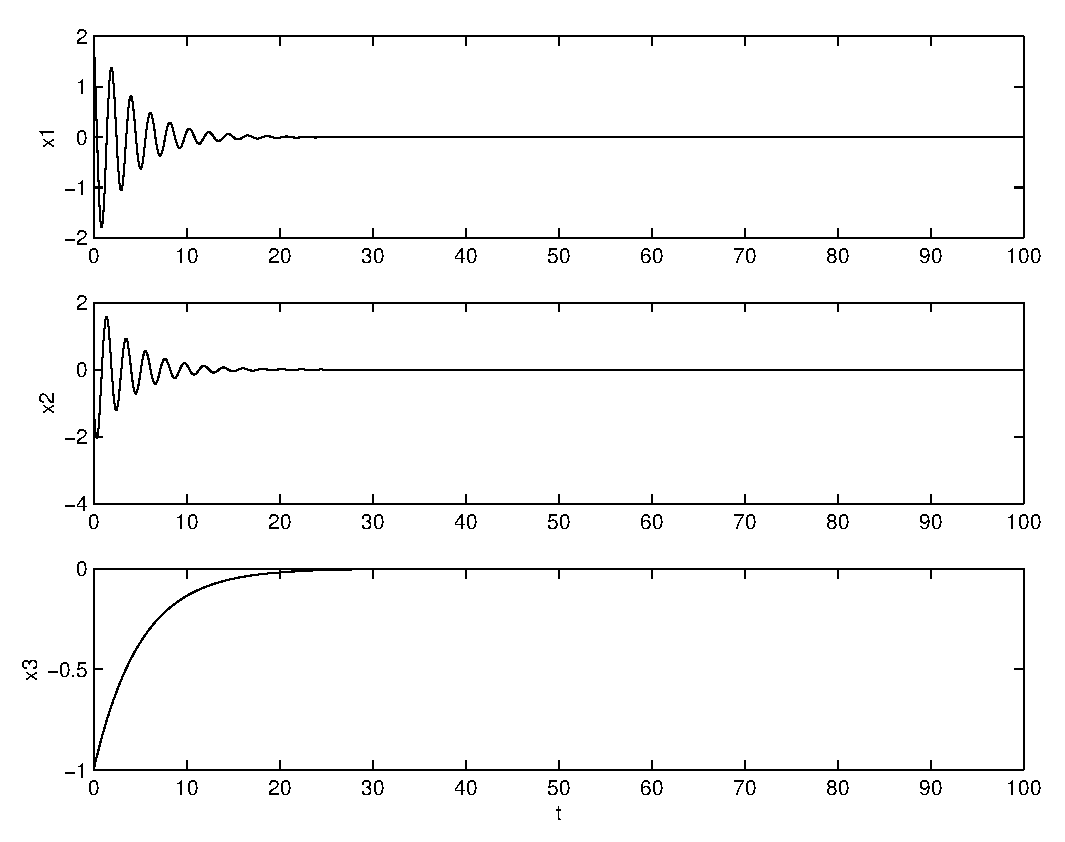
\psfig{file=figures/flinear1.eps,width=5.6in,height=2.8in}}
   \caption{Time series showing convergence to the origin for the solution 
	of the linear system $\dot X=AX$, where $A$ is as in 
	\protect\Ref{E:3dexample}, with initial condition $X_0=(2,-1,-1)$.}
   \label{fig:flinear1}
\end{figure}

In drawing Figure~\ref{fig:flinear1} we have introduced another \Matlab 
graphics command {\tt subplot(m,n,p)}\index{\computer!subplot}.  
The {\tt subplot} command activates one 
subfigure in an $m\times n$ matrix of subfigures.  In this case $m=3$ 
and $n=1$ so that we produce three subfigures arranged vertically.  
The number $p$ indicates which subfigure is the active subfigure --- the 
subfigure to which the {\tt plot} command refers.

The second possibility for the graphical representation of the solution
is the phase space plot.  Here we visualize the curve
$(x_1(t),x_2(t),x_3(t))$ in three dimensional space by typing
\begin{verbatim}
clf
plot3(x(:,1),x(:,2),x(:,3))
xlabel('x1')
ylabel('x2')
zlabel('x3')
\end{verbatim}\index{\computer!clf}\index{\computer!plot3}\index{\computer!xlabel}
\index{\computer!ylabel}\index{\computer!zlabel}
The result is shown in Figure~\ref{fig:flinear2}.  Note that we begin by 
using the \Matlab graphics command {\tt clf} to clear all previous graphics.
\begin{figure}[htb]
   \centerline{%
   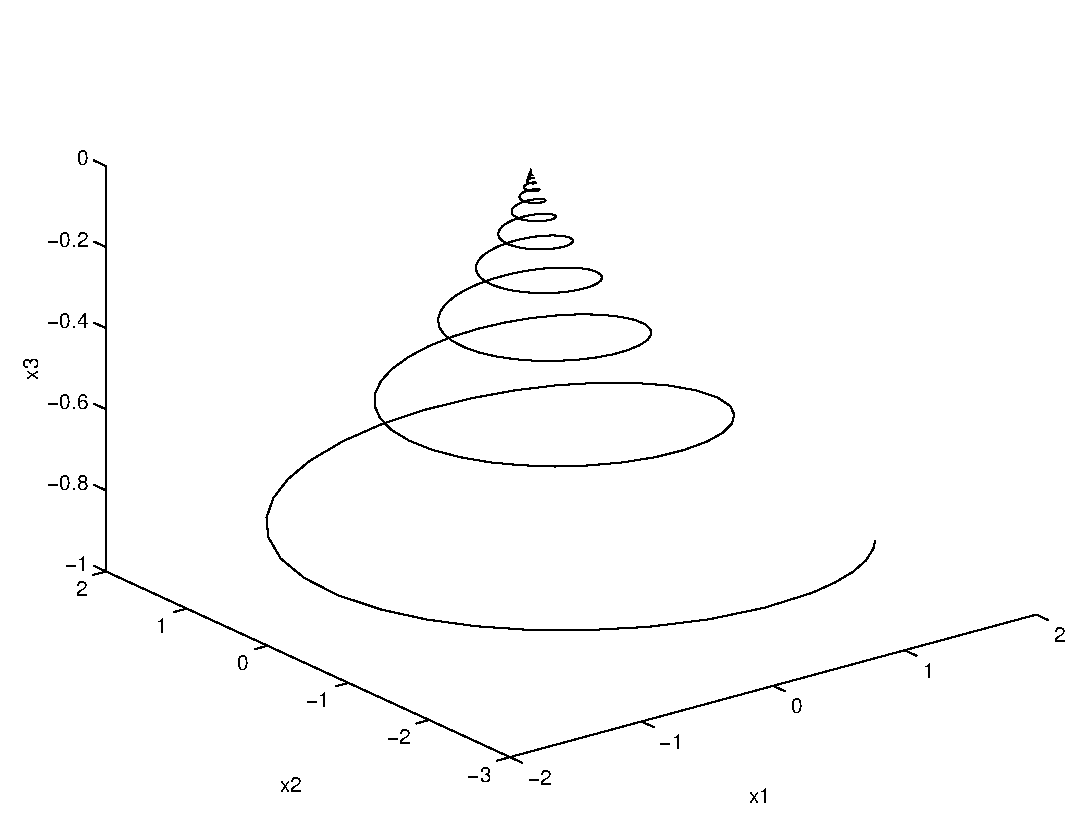
\psfig{file=figures/flinear2.eps,width=3.6in}}
   \caption{Phase space plot showing convergence to the origin for the 
	solution of the linear system $\dot X=AX$, where $A$ is as in 
	\protect\Ref{E:3dexample}, with initial condition $X_0=(2,-1,-1)$.}
   \label{fig:flinear2}
\end{figure}


\subsubsection*{A Three Dimensional Nonlinear System}

We now solve the nonlinear differential equation 
\begin{equation*}  \label{E:fnonlin}
\dot{X} = AX + (2x_1^2 - x_1x_2, -x_3^3, -x_2^2)^t
\end{equation*}
using {\tt ode45} where $A$ is the matrix given in \Ref{E:3dexample}.  The 
m-file for this differential equation is {\tt f14\_4\_3.m}. For completeness, 
this m-file is:
\begin{verbatim}
function f = f14_4_3(t,x)
A = [ -0.25 3.0 0; -3 -0.25 0; 0 0 -0.2];
f = A*x + [2*x(1)^2-x(1)*x(2); -x(3)^3; -x(2)^2];
\end{verbatim}
The theory in Section~\ref{S:QT} guarantees that the origin is
asymptotically stable, and we now verify this statement numerically.  Typing 
\begin{verbatim}
[t,x] = ode45('f14_4_3',[0 100],[0.2,-0.1,-0.1]');
\end{verbatim}
numerically solves this system of ODEs.  The phase space picture, given in
Figure~\ref{F:fnonlin3}, shows convergence to the origin of the nonlinear
system, as expected.  Note the similarity of this figure with the phase
space picture of the linear system given in Figure~\ref{fig:flinear2}. 
These numerical computations are surely in agreement with the conclusion
of Theorem~\ref{T:nlinearization}.

\begin{figure}[htb]
   \centerline{%
   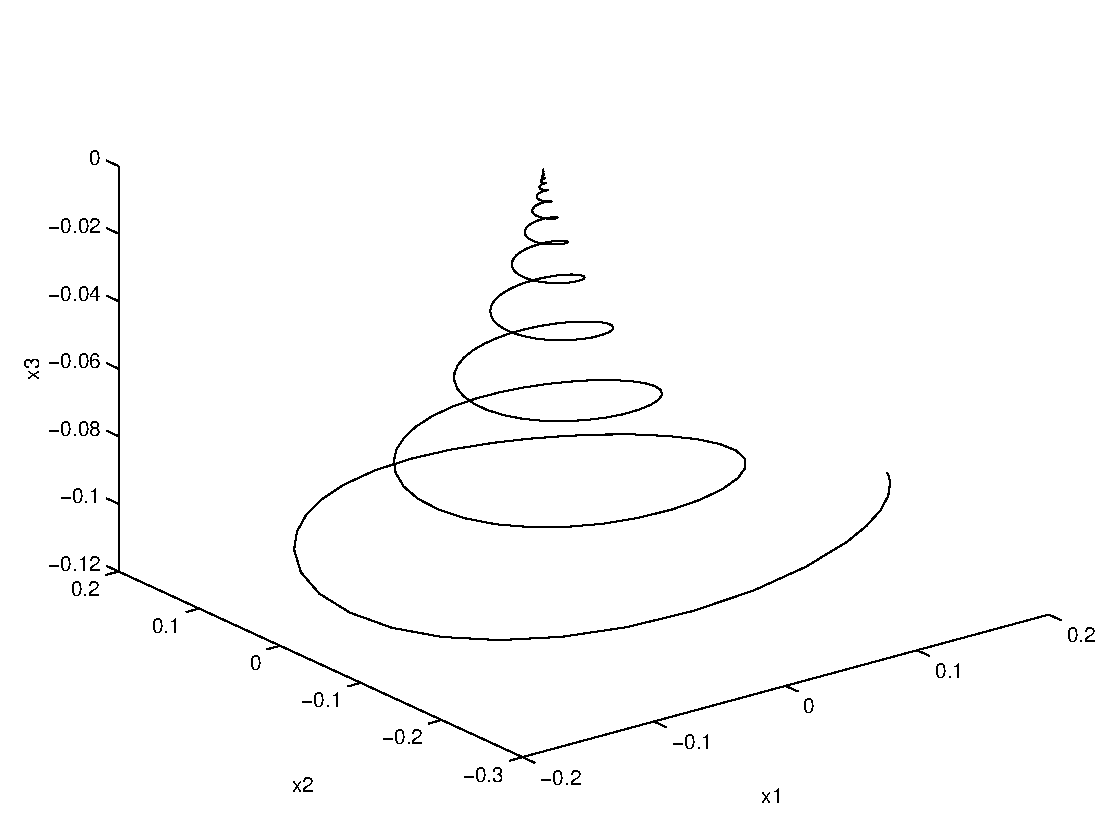
\psfig{file=figures/fnonlin3.eps,width=5.0in}}
   \caption{Time series showing convergence to the origin for the solution of 
	the nonlinear system \protect\Ref{E:fnonlin} with initial condition 
	$X_0=(2,-1,-1)$.}
   \label{F:fnonlin3}
\end{figure}
 
\subsection*{Periodic Solutions in Three Dimensions}

Since planar autonomous nonlinear systems produce limit cycles as solutions, 
it should come as no surprise that nonlinear three-dimensional systems can 
also have periodic solutions.  

An example of a system of differential equations having a limit cycle as a 
solution is:
\begin{equation*} \label{E:3per}
\begin{array}{rcl}
\dot{x}_1 & = & -x_1 - x_2 + x_1x_3 \\
\dot{x}_2 & = &  x_1 - x_2 + x_2x_3 \\
\dot{x}_3 & = &  1 + x_3 - x_1^2 - x_2^2 - x_3^3.
\end{array}
\end{equation*}
Using the m-file
\begin{verbatim}
function f = f14_4_4(t,x)
f = [-x(1) - x(2) + x(1)*x(3); 
      x(1) - x(2) + x(2)*x(3); 
        1  + x(3) - x(1)^2 - x(2)^2 - x(3)^3];
\end{verbatim}
numerically integrate \Ref{E:3per} with initial condition
$X_0=(0.5,0.4,0.3)$ by typing
\begin{verbatim}
[t,x] = ode45('f14_4_4', [0 50], [0.5,0.4,0.3]);
\end{verbatim}
Using {\tt subplot} we can plot the three time series obtaining the result in 
Figure~\ref{F:3per}.  After an initial transient, each component of the 
solution settles into a periodic motion with the same period.
\begin{figure}[htb]
   \centerline{%
   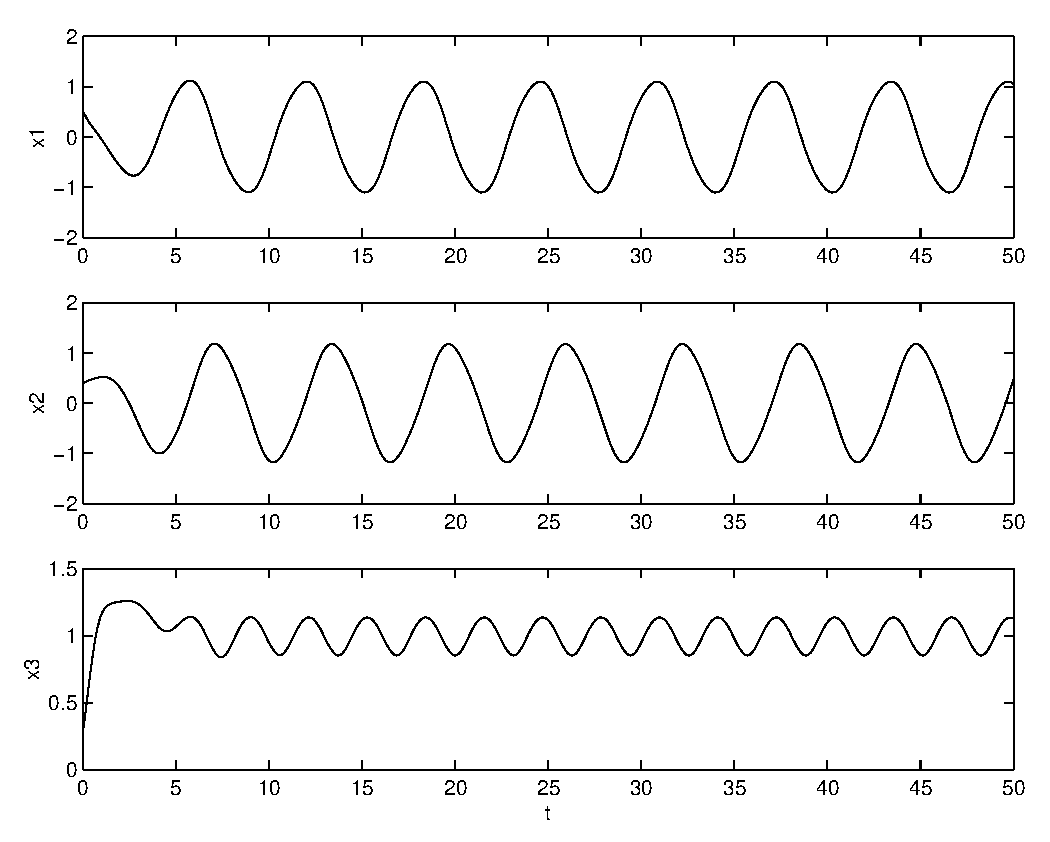
\psfig{file=figures/f3perts.eps,width=3.0in}}
   \caption{Time series showing convergence to a limit cycle for the solution 
	of the nonlinear system \protect\Ref{E:3per} with initial condition 
	$X_0=(0.5,0.4,0.3)$.}
   \label{F:3per}
\end{figure}

In the three-dimensional phase space $x_1,x_2,x_3$ this solution converges to a 
a simple closed curve or a deformed `circle'.  See Figure~\ref{F:3perps} 
which is reproduced using the \Matlab commands
\begin{verbatim}
plot3(x(:,1),x(:,2),x(:,3))                  
xlabel('x1')
ylabel('x2')
zlabel('x3')
\end{verbatim}

\begin{figure}[htb]
   \centerline{%
   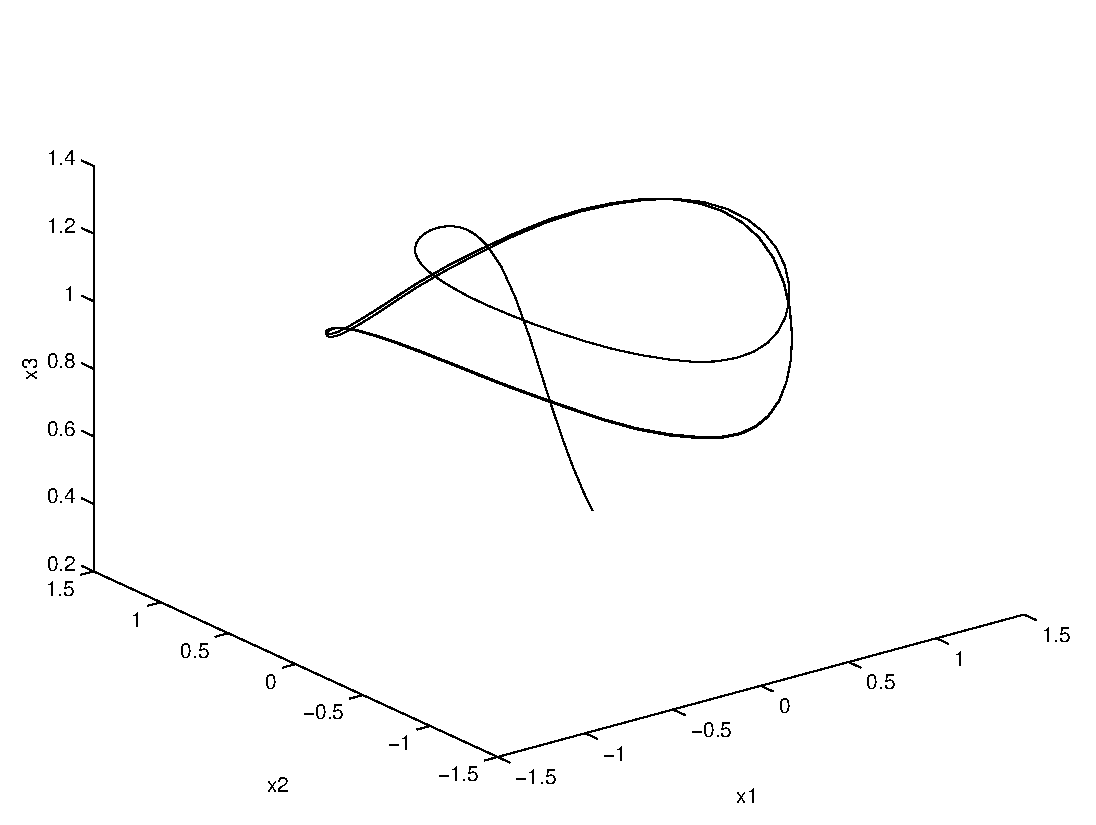
\psfig{file=figures/f3perps.eps,width=3.0in}}
   \caption{Phase space picture showing convergence to a deformed `circle' 
	for the solution of the nonlinear system \protect\Ref{E:3per} with 
	initial condition $X_0=(0.5,0.4,0.3)$.}
   \label{F:3perps}
\end{figure}


\EXER

\CEXER

\noindent In Exercises~\ref{c11.3.1a} -- \ref{c11.3.1b} use linear algebra to 
decide whether or not the origin is an asymptotically stable equilibrium for 
each system of ODEs $\dot{X}=AX$. If the origin is unstable, find an initial 
condition such that the corresponding solution approaches the origin as $t$ 
tends to infinity.  Verify these calculations using {\tt ode45}.
\begin{exercise} \label{c11.3.1a}
\begin{equation*}
A =  \left(\begin{array}{rrrr}
    -5  &  1  & -3  &  0\\
    -2  &  3  & -3  &  0\\
     4  & 11  & -5  &  0\\
     2  & -5  &  3  & -2
\end{array}\right)
\end{equation*}
\end{exercise}
\begin{exercise} \label{c11.3.1b}
\begin{equation*}
A =  \left(\begin{array}{rrrr}
     0  &  1  & -3  &  0\\
    -2  &  3  & -3  &  0\\
     4  & 11  & -5  &  0\\
     2  & -5  &  3  & -2
\end{array}\right).
\end{equation*}
\end{exercise}

\noindent In Exercises~\ref{c11.4.1a} -- \ref{c11.4.1d} investigate
numerically the behavior of solutions of the ODEs in a neighborhood
of the given equilibrium $X_0$.  Based on your observations decide
whether or not the equilibrium is asymptotically stable.

\begin{exercise} \label{c11.4.1a}
Explore the system \Ref{e11.4.1a} near the equilibrium $X_0 = (0,0,0)$:
\begin{equation*}  \label{e11.4.1a}
\begin{array}{rcl}
\dot{x}_1 & = & -x_1 - x_2 + x_2 x_3\\
\dot{x}_2 & = & x_1 - x_2 +x_1^2\\
\dot{x}_3 & = & -x_3 + x_1 x_2
\end{array}.
\end{equation*}
\end{exercise}

\begin{exercise} \label{c11.4.1b}
Explore the system \Ref{e11.4.1b} near the equilibrium $X_0 = (0,0,0)$:
\begin{equation*}  \label{e11.4.1b}
\begin{array}{rcl}
\dot{x}_1 & = & 10(x_2-x_1)\\
\dot{x}_2 & = & 28 x_1 - x_2 - x_1x_3\\
\dot{x}_3 & = & -\frac{8}{3} x_3 + x_1x_2,
\end{array}.
\end{equation*}
\end{exercise}

\begin{exercise} \label{c11.4.1c}
Explore the system \Ref{e11.4.1c} near the equilibrium $X_0 = (1,0,2)$:
\begin{equation*}  \label{e11.4.1c}
\begin{array}{rcl}
\dot{x}_1 & = & 3x_1+x_3-3-x_1x_3\\
\dot{x}_2 & = & x_1 - 1 + x_2x_3\\
\dot{x}_3 & = & x_2 + x_3 -2 + x_1 x_2 - x_2 x_3
\end{array}.
\end{equation*}
\end{exercise}

\begin{exercise} \label{c11.4.1d}
Explore the system \Ref{e11.4.1d} near the equilibrium $X_0 = (0,0,2)$:
\begin{equation*}  \label{e11.4.1d}
\begin{array}{rcl}
\dot{x}_1 & = & -x_1-x_3+3-\cos(x_1)\\
\dot{x}_2 & = & 1-\cos(x_1) - x_3\sin(x_2)\\
\dot{x}_3 & = & 2-x_3 - \sin(x_2)\cos(x_1)
\end{array}.
\end{equation*}
\end{exercise}

\begin{exercise} \label{c11.4.7}
Use \Matlab to verify the conclusion of Theorem~\ref{T:nlinearization}
for the nonlinear differential equation in \Ref{e:fnonlin}.  Choose
the matrix $A$ as in \Ref{eq:fexam4} and the higher order terms $N(X)$
as in \Ref{E:fnonlin1}.
\end{exercise}


\section{Quasiperiodic Motions and Tori}
\label{S:NLD}


In Chapter~\ref{chap:SolveOdes} we saw that in single autonomous differential 
equations the only asymptotically stable solutions are steady-state 
solutions.  In Chapter~\ref{C:NPS} we saw that in two dimensional autonomous
systems the asymptotically stable solutions include limit cycles
\index{limit cycle} as well as equilibria.  In this section and the next we 
show that in higher dimensions asymptotically stable solutions can be even 
more complicated.   Formulas for these complicated solutions cannot be found
analytically; therefore, we use the \Matlab command {\tt ode45}
\index{\computer!ode45} to investigate these solutions.  

In this section we introduce quasiperiodic two-frequency solutions in three 
stages.  First, we discuss quasiperiodic motion\index{motion!quasiperiodic} 
in linear four dimensional systems; second, we discuss asymptotically stable 
quasiperiodic motion in four dimensions; and third we discuss asymptotically
stable quasiperiodic motion in three dimensions.  We also show that
two-frequency quasiperiodic motions fill out a torus (the surface of a
doughnut) as opposed to a point (an equilibrium) or a circle (a periodic 
solution).

\subsection*{A Linear Torus in Four Dimensions}
\index{torus}\index{motion!on a torus}

We know that the origin is a center\index{center} in a linear planar system 
when the eigenvalues are purely imaginary complex conjugates $\pm\tau i$.
All trajectories in a center (except for the origin) lie on ellipses
(or circles) surrounding the origin. We now ask what the geometry 
of solution trajectories is in four dimensional linear systems with 
two pairs of complex conjugate purely imaginary eigenvalues $\pm\tau_1i$
and $\pm\tau_2i$. 

Suppose we start the discussion with a Jordan normal form\index{Jordan normal form} 
matrix 
\[
B = \left(\begin{array}{rrrr}
  0  &  -0.1  &  0   &  0       \\
0.1  &    0   &  0   &  0       \\
  0  &    0   &  0   & \sqrt{23}\\
  0  &    0   & -\sqrt{23} & 0
\end{array}\right).
\]
The associated linear system decouples into two planar systems
\[
\begin{array}{rcl}
\dot{x}_1 & = & -0.1x_2 \\
\dot{x}_2 & = &  0.1x_1 \\
\end{array}
\AND
\begin{array}{rcl}
\dot{x}_3 & = &  \sqrt{23}x_4 \\
\dot{x}_4 & = & -\sqrt{23}x_3 \\
\end{array}.
\]
Since each of these systems is a center\index{center} (in normal form) the phase 
plane of each system consists of concentric circles.  

Suppose that $(x_1(t),x_2(t),x_3(t),x_4(t))$ is a solution to the 
four dimensional system.  Then $(x_1(t),x_2(t))$ is a solution to the 
first planar system and $(x_3(t),x_4(t))$ is a solution to the second 
planar system.  Since we know what phase portraits
\index{phase!portrait!for a center} and time series for
centers look like, we conclude that each of the time series $x_j(t)$ is
a periodic function (in fact just a sum of a cosine and a sine function).  
The only difference between these functions is the frequency that is 
$0.1$ for the first two time series and $\sqrt{23}=4.7958$ for the third 
and fourth time series.

We ask:  Is this description accurate for the general four dimensional linear 
system with two pairs of purely imaginary complex conjugate eigenvalues?  The 
answer is NO and the answer is interesting.  The general solution
\index{general solution} to such an equation lives on a torus\index{torus} 
(the surface of a doughnut) and the general times series is quasiperiodic
\index{motion!quasiperiodic} 
with two frequencies\index{frequency}.  Linear algebra 
tells us that by simply changing coordinates we can put the matrix into 
Jordan normal form\index{Jordan normal form}.  So if the information about 
solutions that we have just described is accurate, the complication must come 
from viewing the solutions in a different coordinate system.

We do this as follows.  Let
\[
P = \left(\begin{array}{rrrr}
   -2  &  1   &  3  &  4 \\
   -1  &  2   &  2  &  1 \\
    1  &  4   &  1  &  0\\
    0  &  0   &  2  &  1
\end{array}\right)
\]
and note that $\det(P)=27$ so that $P$ is invertible\index{invertible}.  
Now let
$A=PBP\inv$ so that $A$ is just a matrix whose 
Jordan normal form\index{Jordan normal form} is $B$.
A calculation (using \Matlabp) shows that
\begin{equation*}  \label{e:tor4}
A = \left(\begin{array}{rrrr}
   10.6722 &  -16.0417 &    5.4028 &  -12.2597\\
    5.3472 &   -8.1375 &    2.7569 &   -3.6597\\
    2.1574 &   -3.5194 &    1.1954 &   -0.3144\\
    5.3287 &   -7.9931 &    2.6644 &   -3.7301
\end{array}\right).
\end{equation*}
By typing
\begin{verbatim}
e14_5_1
eig(A)
\end{verbatim}\index{\computer!eig}
we can check that the eigenvalues of $A$ are $\pm0.1i$ and $\pm\sqrt{23}i$.

We now compute the solution to the corresponding linear system of ODEs 
$\dot{X}=AX$ where the function {\tt A*x} is stored in the m-file 
{\tt f14\_5\_1} on the time interval $[0,100]$ with 
initial conditions $X_0=(0.2,0.6,-0.5,0.1)$. Type
\begin{verbatim}
[t,x] = ode45('f14_5_1',[0 100],[0.2,0.6,-0.5,0.1]');
\end{verbatim}\index{\computer!ode45}
Using the \Matlab instruction {\tt subplot} described in 
Section~\ref{S:ode45HD}, we can graph the four time series\index{time series}.
The results are given in 
Figure~\ref{F:ftor4ts}.  Note how the time series oscillate on both a short 
scale and on a long scale --- one scale corresponding to each frequency.  
These trajectories\index{trajectory} are called {\em quasiperiodic\/}
\index{motion!quasiperiodic} or {\em two frequency\/} motions.
\index{motion!two frequency}  Trajectories with many frequencies can be 
found in yet higher dimensional linear systems.


\begin{figure}[htb]
   \centerline{%
   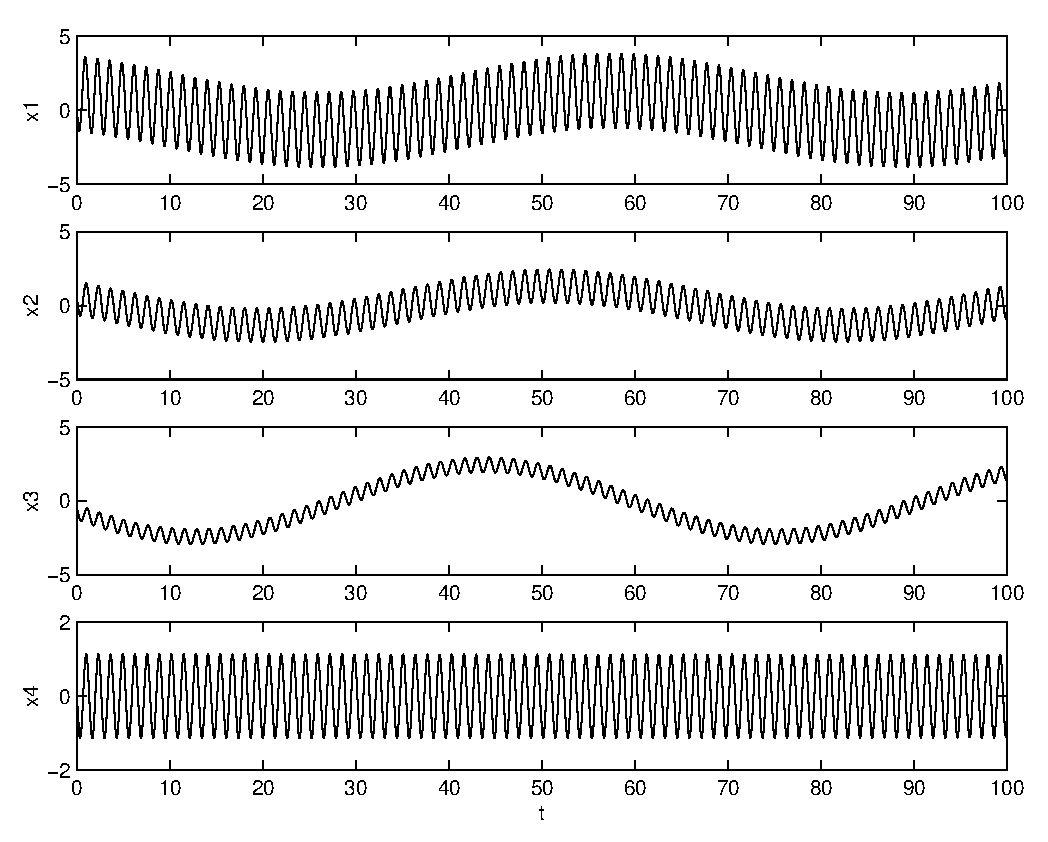
\psfig{file=figures/ftor4ts.eps,width=5.3in}}
   \caption{Time series showing quasiperiodic two-frequency motion for the 
	solution of the linear system \protect\Ref{e:tor4} with initial 
	condition $X_0=(0.2,0.6,-0.5,0.1)$.}
   \label{F:ftor4ts}
\end{figure}

The phase space portrait can be viewed in three dimensions (by just 
ignoring one coordinate).  The projections of this trajectory onto the 
$x_1x_3x_4$ hyperplane and the $x_1x_2x_4$ hyperplanes are given in 
Figure~\ref{F:ftorphase}.  There we can see the torus\index{torus}.  For 
linear systems with two pairs of complex conjugate purely imaginary
eigenvalues, almost all solutions lie on tori.  To verify this statement, 
experiment with different initial conditions and see Exercise~\ref{EX:tor4}. 

\begin{figure}[htb]
   \centerline{%
   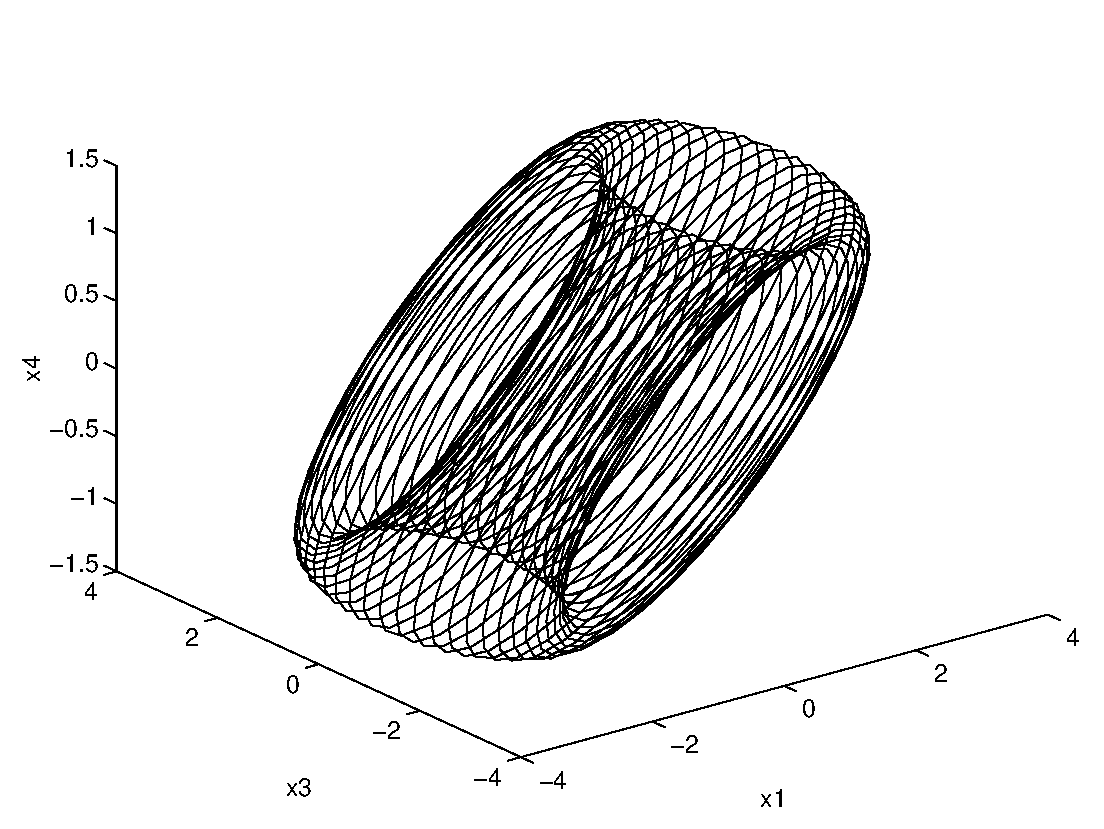
\psfig{file=figures/ftor4ps1.eps,width=3.0in}
   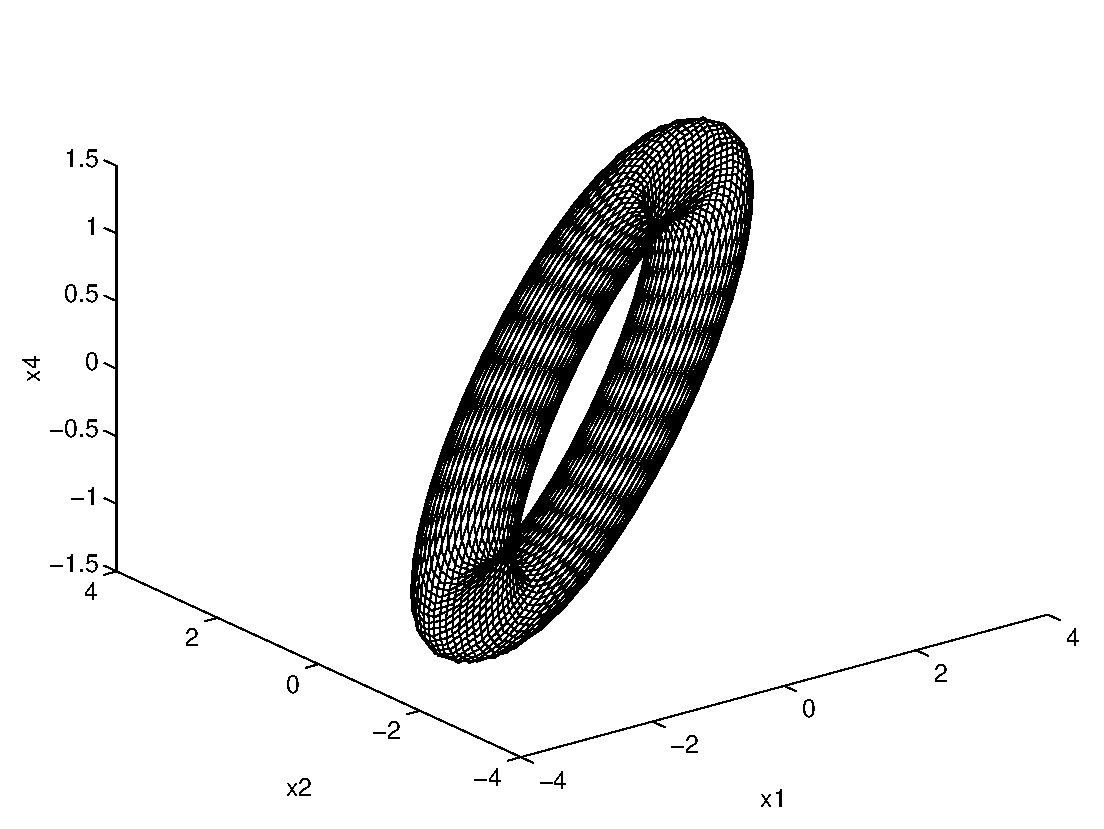
\psfig{file=figures/ftor4ps2.eps,width=3.0in}}
   \caption{Phase space projections showing quasiperiodic motion on a torus of 
	the solution of the linear system \protect\Ref{e:tor4} with initial 
	condition $X_0=(0.2,0.6,-0.5,0.1)$.}
   \label{F:ftorphase}
\end{figure}

\subsection*{Asymptotically Stable Quasiperiodic Motion}
\index{motion!quasiperiodic}

In Section~\ref{S:HopfBif} we discussed Hopf bifurcation of planar autonomous 
systems that leads, by varying a parameter through a center, to an 
asymptotically stable periodic trajectory.  Here we discuss how we can also 
find asymptotically stable quasiperiodic motions\index{motion!quasiperiodic} 
in a similar way.  

\subsubsection*{Motion on a Torus in Four Dimensions}
\index{torus!in dimension four}

Consider the system of four differential equations 
\begin{equation*}  \label{e:nonlintor}
\dot{X} = (A+\epsilon I_4)X - ||X||^2X,
\end{equation*}
where $A$ has two pairs of complex conjugate purely imaginary eigenvalues
and $\epsilon>0$.  We see that $X=0$ is an equilibrium for \Ref{e:nonlintor}
and the Jacobian\index{matrix!Jacobian} 
matrix is $A+\epsilon I_4$ whose eigenvalues 
are $\lambda+\epsilon$ where $\lambda$ is an eigenvalue of $A$.  Since all 
of the eigenvalues of the Jacobian have positive real part, the origin is a 
source\index{source} in four dimensions.  On the other hand, the term 
$-||X||^2X$ in \Ref{e:nonlintor} always drives solutions toward the origin. 
The two forces balance and result in one asymptotically stable invariant 
torus.   The reasoning here is similar to that used to find limit cycles in
planar phase/amplitude equations.

Let $A$ be the matrix \Ref{e:tor4} and solve numerically the corresponding
differential equation \Ref{e:nonlintor} using the preloaded m-file 
{\tt f14\_5\_2.m}. That m-file is:
\begin{verbatim}
function f = f14_5_2(t,x)
A = [ 10.6722 -16.0417   5.4028 -12.2597;
       5.3472  -8.1375   2.7569  -3.6597;
       2.1574  -3.5194   1.1954  -0.3144;
       5.3287  -7.9931   2.6644  -3.7301];
f = (A+0.1*eye(4))*x - norm(x)^2*x;
\end{verbatim}\index{\computer!norm}
To solve this differential equation with initial conditions 
$X_0=(0.2,0.6,-0.5,0.1)$, type
\begin{verbatim}
[t,x] = ode45('f14_5_2',[0 100],[0.2,0.6,-0.5,0.1]');
\end{verbatim}\index{\computer!ode45}

The time series for this nonlinear system are given in Figure~\ref{F:tornlts}.
Note the initial transient that is present before the solution settles 
down to a quasiperiodic motion\index{motion!quasiperiodic} on a torus.
\index{torus}  The phase space picture in the $x_1x_3x_4$ hyperplane is given 
in Figure~\ref{F:tornlps}.  Here the transient is more visible.
 
\begin{figure}[htb]
   \centerline{%
   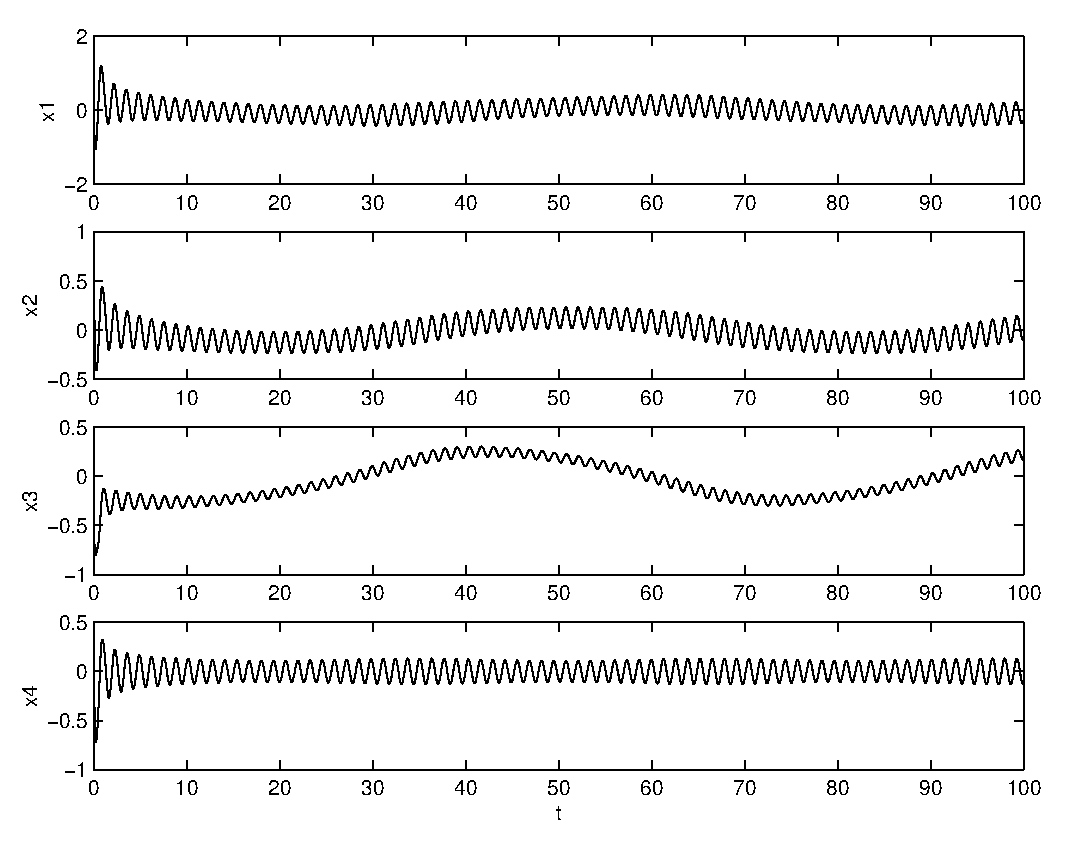
\psfig{file=figures/ftornlts.eps,width=5.3in}}
   \caption{Time series showing quasiperiodic two-frequency motion for the 
	solution of the nonlinear system \protect\Ref{e:nonlintor} with 
	initial condition $X_0=(0.2,0.6,-0.5,0.1)$.}
   \label{F:tornlts}
\end{figure}

\begin{figure}[htb]
   \centerline{%
   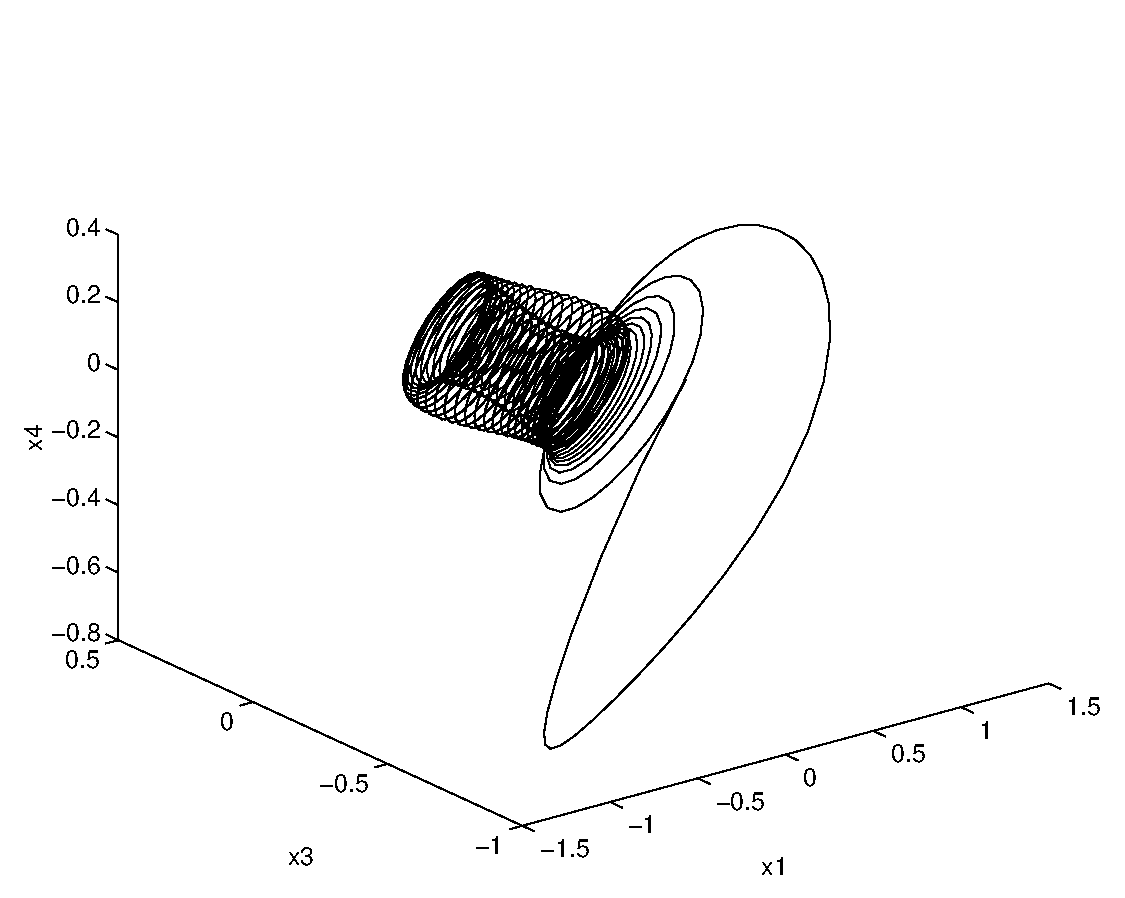
\psfig{file=figures/ftornlps.eps,width=5.0in}}
   \caption{Phase space projections showing motion on a torus for the 
	solution of the nonlinear system \protect\Ref{e:nonlintor} with 
	initial condition $X_0=(0.2,0.6,-0.5,0.1)$.}
   \label{F:tornlps}
\end{figure}



\subsubsection*{A Torus in Three Dimensions}
\index{torus!in dimension three}

Until now, the way that we have constructed two frequency quasiperiodic 
solutions to systems of ODEs is based on having two independent frequencies 
present in a linear system.  It is not obvious --- yet it is true --- 
that solutions to nonlinear systems of three differential equations 
can also have two frequency quasiperiodic 
solutions\index{motion!two frequency}.  The theory that 
leads to this example is beyond the scope of this book; nevertheless, we
now have the numerical techniques to see (visually) that such solutions 
exist.

Consider the autonomous nonlinear system of ODEs\footnote{This system of
equations is taken from W.F. Langford, Numerical studies of torus bifurcations, 
ISNM {\bf 70}, Birkh\"auser, 1984.}:
\begin{equation*}  \label{e:ftor3}
\begin{array}{rcl}
\dot{x}_1 & = & (x_3-0.7)x_1 - 3.5x_2\\
\dot{x}_2 & = &  3.5x_1 + (x_3-0.7)x_2 \\
\dot{x}_3 & = & 0.6 + x_3 - 0.33x_3^3 - (x_1^2+x_2^2)(1+.25x_3).
\end{array}
\end{equation*}
The m-file for this system of equations is 
{\tt f14\_5\_3.m} and contains
\begin{verbatim}
function f = f14_5_3(t,x)
f = [(x(3)-0.7)*x(1) - 3.5*x(2); 
     3.5*x(1) + (x(3)-0.7)*x(2); 
     0.6 + x(3) - x(3)^3/3 - (x(1)^2+x(2)^2)*(1+0.25*x(3))];
\end{verbatim}
The differential equation \Ref{e:ftor3} is solved by typing
\begin{verbatim}
[t,x] = ode45('f14_5_3',[0 100],[0.1,0.03,0.001]');
\end{verbatim}\index{\computer!ode45}
The time series for the system \Ref{e:ftor3} are given in 
Figure~\ref{F:tor3ts} and the three dimensional phase space
\index{phase!space} picture is given in Figure~\ref{F:tor3ps}.

\begin{figure}[htb]
   \centerline{%
   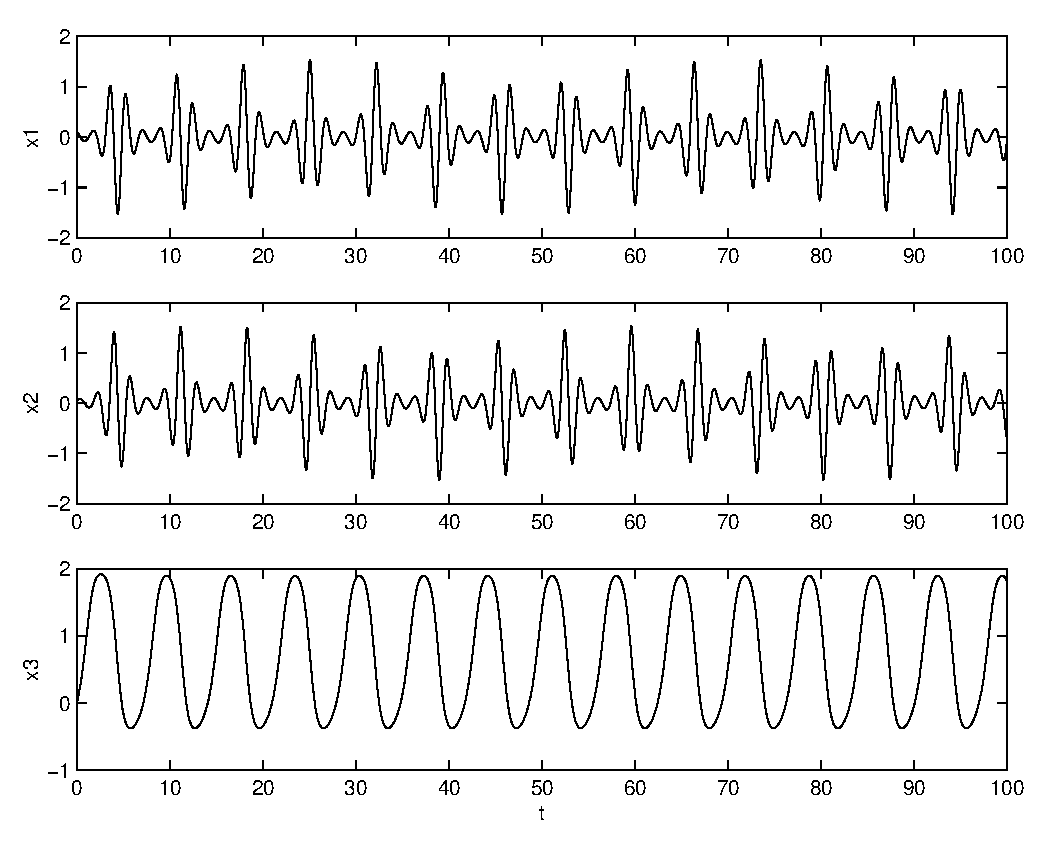
\psfig{file=figures/ftor3ts.eps,width=5.0in}}
   \caption{Time series showing quasiperiodic two-frequency motion for the 
	solution of the nonlinear system \protect\Ref{e:ftor3} with initial 
	condition $X_0=(0.1,0.03,0.001)$.}
   \label{F:tor3ts}
\end{figure}

\begin{figure}[htb]
   \centerline{%
   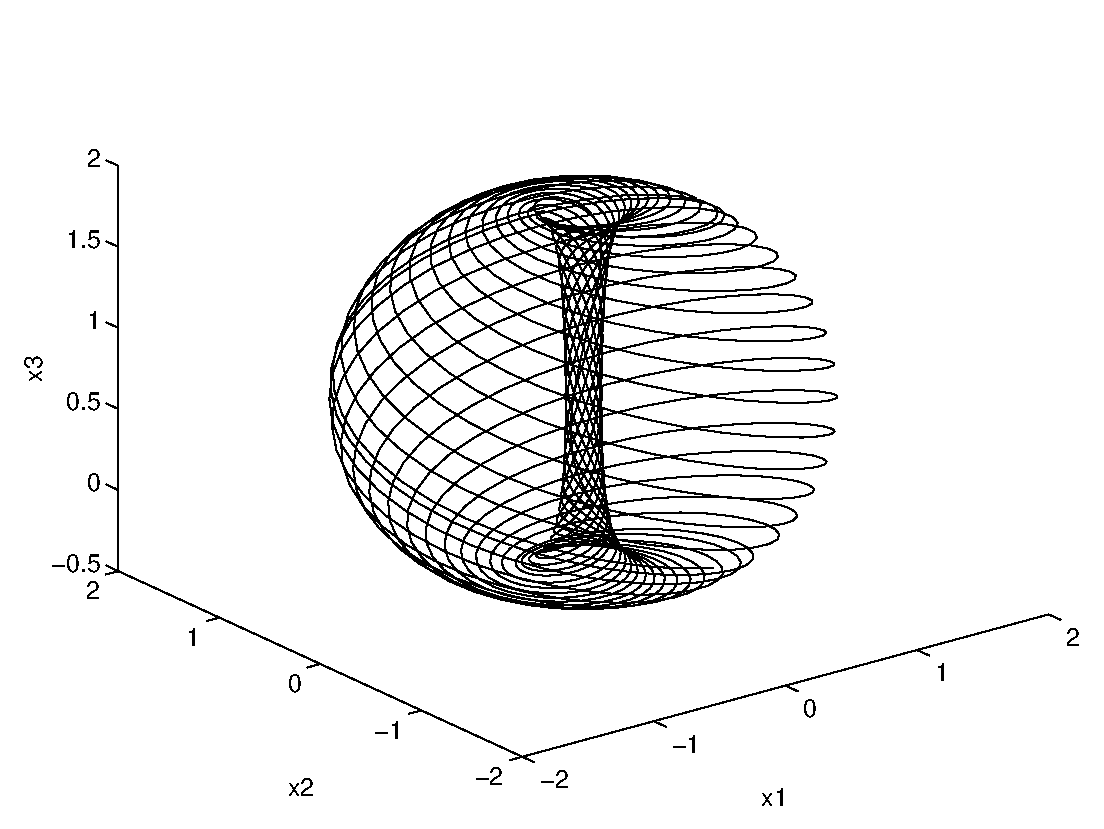
\psfig{file=figures/ftor3ps.eps,width=5.0in}}
   \caption{Phase space showing motion on a torus for the solution trajectory 
	of the nonlinear system \protect\Ref{e:ftor3} with initial condition 
	$X_0=(0.1,0.03,0.001)$.}
   \label{F:tor3ps}
\end{figure}


\EXER

\CEXER

\begin{exercise}  \label{EX:tor4}
Let A be the $4\times 4$ torus example given in \Ref{e:tor4}.  Choose three 
different initial conditions to the system of ODEs $\dot{X}=AX$ and use 
{\tt ode45} compute solutions with these initial conditions.  (To decrease 
the length of time needed by the computer to do these calculations, shorten 
the time period to say $[0,30]$.)  
\begin{itemize}
\item[(a)]  Based on these calculations, verify that most initial conditions 
lead to quasiperiodic toroidal motions.  Display both time series and 
three dimensional phase portraits of your solutions. 
\item[(b)]  Take as initial condition the real part of one of the complex
eigenvectors of $A$.  (You will need to use \Matlab to find the eigenvalues
and eigenvectors of $A$.)  What kind of phase space motion do you see now? 
How does this solution differ from the toroidal motions obtained in (a)? 
Use Jordan normal forms to explain why your numerical answer is correct.
\end{itemize}
\end{exercise} 

\noindent In Exercises~\ref{c14.5.2a} -- \ref{c14.5.2d} use \Matlab to find
out whether the system of differential equations $\dot X= AX$ for
the given matrix $A$ has quasiperiodic solutions.
\begin{exercise} \label{c14.5.2a}
\begin{equation*}
A=\left(\begin{array}{rrrr}
    4.9666  &  2.2833  &  0.8000  &  5.3666\\
   -0.9889  & -0.0944  & -1.6000  & -1.7889\\
    2.9889  &  4.0944  & -0.4000  &  1.7889\\
   -8.9443  & -4.4721  &       0  & -4.4721
\end{array}\right).
\end{equation*}
\end{exercise}

\begin{exercise} \label{c14.5.2b}
\begin{equation*}
A=\left(\begin{array}{rrrr}
    2.7666  &  0.2833  &  1.4000  &  4.5666\\
    2.4111  &  1.9056  & -1.8000  & -0.1889\\
   -0.4111  &  2.0944  & -0.2000  &  0.1889\\
   -7.9443  & -2.4721  & -1.0000  & -4.4721
\end{array}\right).
\end{equation*}
\end{exercise}

\begin{exercise} \label{c14.5.2c}
\begin{equation*}
A=\left(\begin{array}{rrrrr}
    0.7130  & 24.8184  & 32.0740  &  2.8959  & 15.3610\\
    0.0552  & 17.0732  & 21.1395  &  6.6120  & 11.0843\\
   -0.6168  &-12.0764  &-16.0165  & -1.6151  & -7.3997\\
    1.0410  & -3.3312  & -2.0820  & -3.3312  & -3.1230\\
   -0.5205  &  1.6656  &  1.0410  &  1.6656  &  1.5615
\end{array}\right).
\end{equation*}
\end{exercise}

\begin{exercise} \label{c14.5.2d}
\begin{equation*}
A=\left(\begin{array}{rrrrr}
  -10.2870 &  40.8184 &  30.0740 &  19.8959 &  38.3610\\
   -7.4448 &  25.0732 &  16.1395 &  15.8620 &  26.0843\\
    6.8833 & -20.0764 & -11.0165 & -10.3652 & -21.3998\\
    1.0410 &  -3.3312 &  -2.0820 &  -3.3312 &  -3.1230\\
   -0.5205 &   1.6656 &   1.0410 &   1.1656 &   0.5615
\end{array}\right).
\end{equation*}
\end{exercise}


\section{Chaos and the Lorenz Equation}
\label{S:chaos} \index{chaos}\index{Lorenz system}


Classifying all of the kinds of solutions that can occur asymptotically in 
autonomous systems of first order differential equations is a difficult task 
and is very much a topic of current research.  Until now we have discussed 
three types of solutions: equilibria, limit cycles, and quasiperiodic
motions.  The purpose of the next example, the Lorenz equations, is to 
illustrate that there are still other types of asymptotic behavior that can 
occur in solutions to autonomous ordinary differential equations in three 
dimensions.  This type of solution is called {\em chaotic\/} and what 
distinguishes chaotic solutions from the previously discussed solutions is 
{\em sensitive dependence on initial conditions\/}. \index{chaos}

The prototypical example of chaos is the {\em Lorenz system}. 
\index{Lorenz system}  The Lorenz system consists of three first order 
(almost linear) ordinary differential equations (there are just two quadratic 
terms):
\begin{equation*}  \label{e:Lorenz}
\begin{array}{rcl}
\dot{x}_1 & = & \sigma(x_2-x_1)\\
\dot{x}_2 & = & \rho x_1 - x_2 - x_1x_3\\
\dot{x}_3 & = & -\beta x_3 + x_1x_2,
\end{array}
\end{equation*}
where $\sigma$, $\rho$ and $\beta$ are real constants.  We consider here
solutions to \Ref{e:Lorenz} when
\[
\sigma=10,\quad \beta=\frac{8}{3},\quad \rho=28.
\]
The right hand side of \Ref{e:Lorenz} is stored in the m-file {\tt f14\_6\_1.m}:
\begin{verbatim}
function f = f14_6_1(t,x)
sigma = 10;  beta  = 8/3;  rho   = 28;
f     = [sigma*(x(2)-x(1));
         rho*x(1)-x(2)-x(1)*x(3);
         -beta*x(3)+x(1)*x(2)];
\end{verbatim}

\begin{figure}[bht]
   \centerline{%
   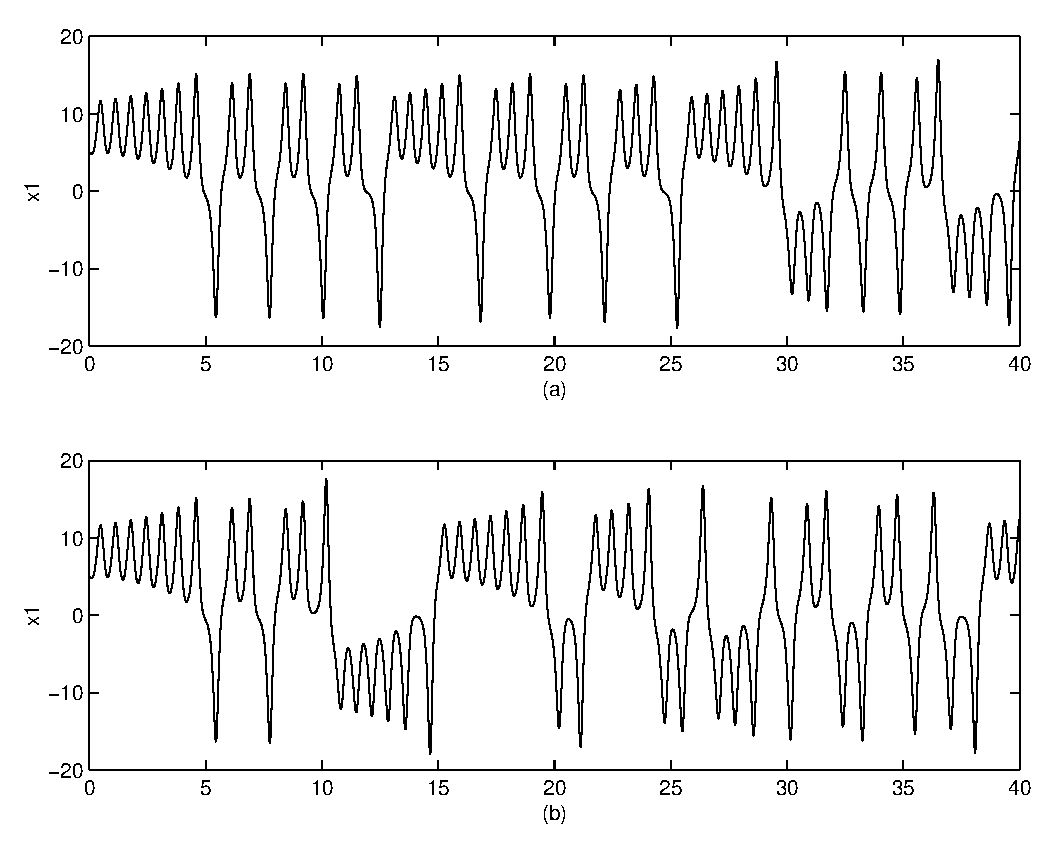
\psfig{file=figures/lorenz12.eps,width=3.0in}}
   \caption{Approximation of chaotic solutions of the Lorenz system by 
	{\tt ode45} illustrating sensitive dependence on initial conditions.  
	(a) A solution starting at $(5,5,30)$;  (b) a solution starting at 
	$(5.01,5,30)$.}
   \label{fig:lorenz1}
\end{figure}

Compute a solution of the Lorenz system\index{Lorenz system} starting at 
$X_0=(5,5,30)$ by typing
\begin{verbatim}
[t,x]=ode45('f14_6_1',[0 40],[5,5,30]');
\end{verbatim}
The time series of $x_1$ is shown in Figure~\ref{fig:lorenz1}(a).  This time 
series looks bizarre and no apparent regularity can be seen.  Moreover, the 
motion is not just irregular, it is also sensitive to the choice of the initial 
conditions.  \index{sensitivity to initial conditions}


\subsubsection*{Sensitive Dependence on Initial Conditions}

In Figure~\ref{fig:lorenz1}(b) we illustrate sensitive dependence by showing  
a solution of the Lorenz system\index{Lorenz system} with initial conditions 
very close to the first one, namely at $X_0=(5.01,5,30)$.  In the beginning 
the solutions behave in a similar way, but by $t\approx 10$ the behavior is 
completely different.  Even for smaller 
differences in the initial conditions, the phenomenon of sensitivity to 
initial conditions is still present, although the significant difference in 
the trajectories occurs at a later time (see Figure~\ref{fig:lorenz2}).  

\begin{figure}[htb]
   \centerline{%
   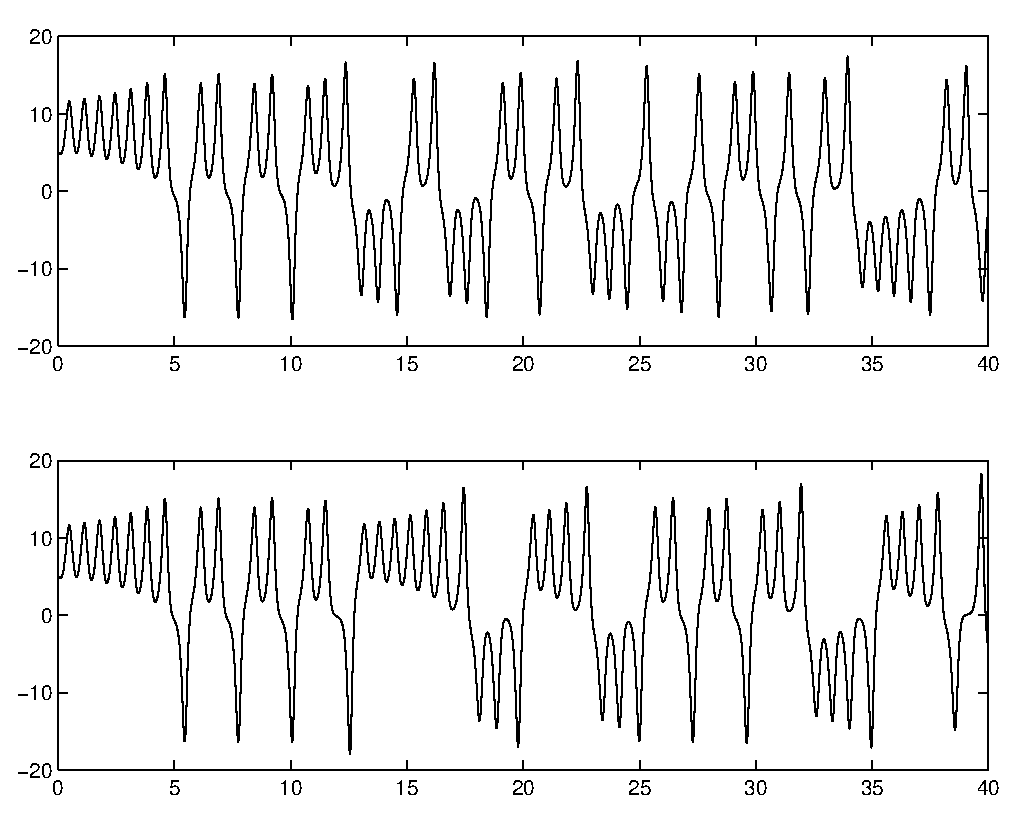
\psfig{file=figures/lorenz34.eps,width=3.0in}}
   \caption{Approximation of chaotic solutions of the Lorenz system by 
	{\tt ode45} illustrating sensitive dependence on initial conditions.
 	 (a) A solution starting at $(5.001,5,30)$;
  	 (b) a solution starting at $(5.0001,5,30)$.}
   \label{fig:lorenz2}
\end{figure}

The consequence of sensitive dependence of solutions on initial conditions in 
the Lorenz system is in long term unpredictable behavior.  Typically, in
experiments, we know initial conditions only to within some (hopefully) small
error.  If these errors get magnified, as they do in the Lorenz system, then
it is impossible to make accurate long term predictions.  This lack of
predictability is the defining feature of {\em chaotic behavior}.
\index{chaos}  So we must ask:  Is chaotic behavior typical in solutions to
autonomous systems of differential equations?  The answer is yes.  Not every
three dimensional systems of differential equations exhibits chaos --- but
many do.  

In Figure~\ref{fig:lorenz3} we show a phase space plot of the
solution starting at $(5,5,30)$.  To reproduce this figure with the 
correct scale and view point type
\begin{verbatim}
[t,x]=ode45('f14_6_1',[0 40],[5,5,30]');
plot3(x(:,1),x(:,2),x(:,3))
axis([-20,20,-20,20,0,60])
view(125,20)
\end{verbatim}\index{\computer!plot3}\index{\computer!axis}\index{\computer!view}
\begin{figure}[htb]
   \centerline{%
   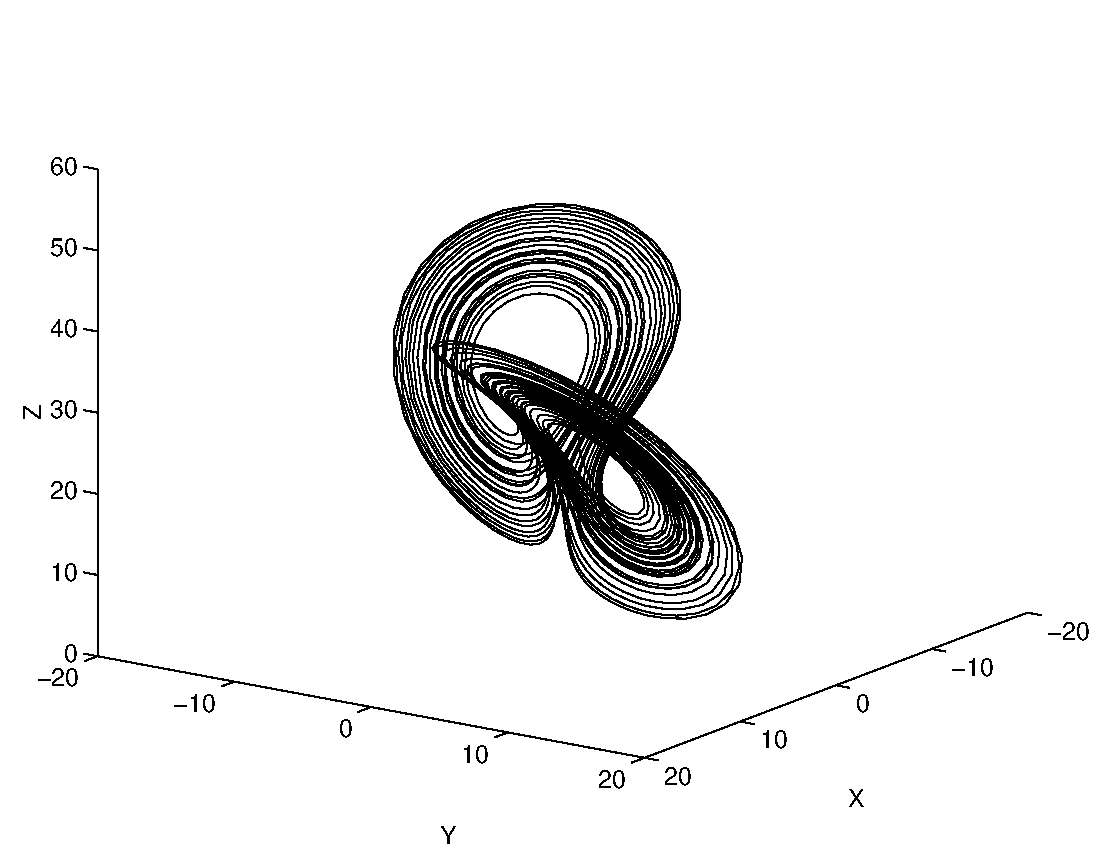
\psfig{file=figures/lorenz5.eps,width=5.5in}}
   \caption{Phase space plot of a solution of the Lorenz system
   starting at $(5,5,30)$.}
   \label{fig:lorenz3}
\end{figure}

We emphasize that the existence of sensitive dependence on initial conditions 
does {\em not\/} depend on the numerical algorithm used in the numerical 
integration nor does it depend on the computer that is used.  However, 
different numerical algorithms and even different computers will give 
different numerical results.   Finally, we note that the phase space picture 
of the Lorenz attractor\index{Lorenz attractor}, as shown in 
Figure~\ref{fig:lorenz3}, will seem the same to the eye, independent of the 
choice of numerical algorithm and computer,
even though the time series will have readily observable differences of the
type shown in Figure~\ref{fig:lorenz2}.  {\bf Remark:}  A dynamic simulation 
of a solution to the Lorenz equations in phase space can also be seen in 
\Matlabp: just type {\tt lorenz}.\index{\computer!lorenz}

It should be noted that even though quasiperiodic motion is geometrically 
complicated (leading to trajectories lying on a torus), it does not exhibit
sensitive dependence on initial conditions.  More precisely, the time series 
of asymptotically stable quasiperiodic solutions remain almost unchanged 
after small changes in initial conditions.  To verify this statement, we 
return to the numerical solution of \Ref{e:ftor3}.  In Figure~\ref{F:tor3tsab}
we plot the time series for the $x_1$ component of solutions with nearly 
identical initial conditions and note that the two time series are nearly 
identical.

\begin{figure}[htb]
   \centerline{%
   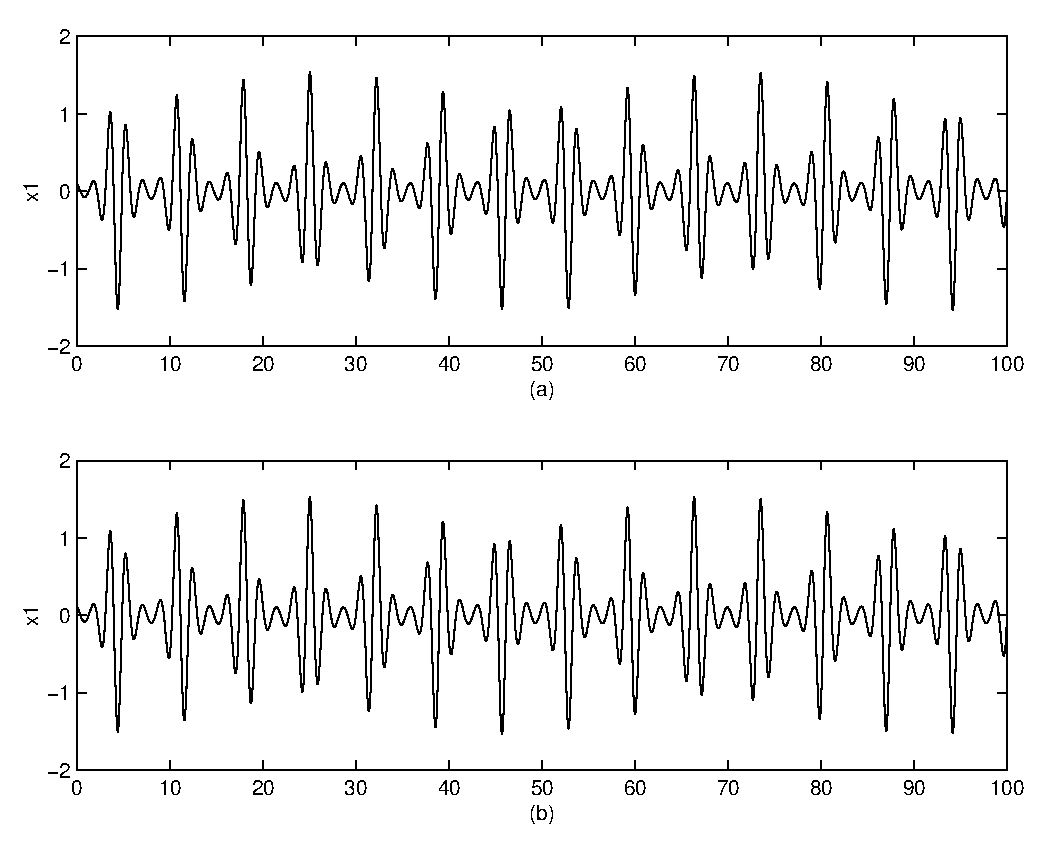
\psfig{file=figures/ftor3tsab.eps,width=3.0in}}
   \caption{Time series for a quasiperiodic two-frequency solution of the 
	nonlinear system \protect\Ref{e:ftor3} illustrating a lack of sensitive 
	dependence on initial conditions: (a) $X_0=(0.1,0.03,0.001)$ and (b) 
	$X_0=(0.11,0.031,0.0015)$.}
   \label{F:tor3tsab}
\end{figure}

\subsection*{A Summary of Observed Three-Dimensional Dynamics}

We now summarize the types of attracting solutions that we have seen in
autonomous three-dimensional systems of differential equations.  The states
we have studied are stable equilibria (or sinks), attracting limit cycles,
attracting quasiperiodic two-frequency motions, and chaotic dynamics such as
seen in the Lorenz equations.  Each of these solution types has well-defined
characteristics that can be observed either in time series plots or in
three-dimensional phase space plots.  This information is summarized in 
Table~\ref{T:assdyn}.

\begin{table}
\begin{center}
\begin{tabular}{|c|c|c|}
\hline
\begin{minipage}[t]{1.1in}
\begin{center}
Asymptotic \\
Solution Type 
\end{center}
\end{minipage}
& Times Series & Phase Space \\
\hline
\hline
sink 
&
horizontal line
&
point \\
\hline
limit cycle
&
periodic oscillation 
&
`circle'
\\ \hline
\begin{minipage}[t]{1.0in}
\begin{center}
two-frequency \\
quasiperiodic 
\end{center}
\end{minipage}
& 
modulated periodic oscillation 
& 
torus
\\ \hline
chaotic 
&
\begin{minipage}[t]{2.3in}
\begin{center}
bounded irregular oscillation \\ 
{\bf with} sensitive dependence \\
on initial conditions
\end{center}
\end{minipage}
&
\begin{minipage}[t]{1.7in}
\begin{center}
complicated surface \\
{\bf not} sensitive \\
to initial conditions
\end{center}
\end{minipage}
\\ \hline
\end{tabular}
\end{center}
\caption{Summary of Observed Asymptotic Dynamics in Three Dimensions}
\label{T:assdyn}
\end{table} 

In Figure~\ref{fig:flinear1} we plotted the time series of a solution to a 
linear equation $\dot{X}=AX$ where the $3\times 3$ matrix $A$ had eigenvalues
with negative real part.  These time series showed convergence to the 
equilibrium at the origin by becoming horizontal as $t$ increased.  There was
transient oscillation caused by a complex conjugate pair of eigenvalues in 
$A$.  The three-dimensional phase portrait Figure~\ref{fig:flinear2} indicates
convergence of this solution trajectory to a point.  These types of time 
series and phase portraits are equally valid for nonlinear systems near a sink,
as was illustrated in Figure~\ref{F:fnonlin3} for the nonlinear system \Ref{E:fnonlin}.

In example \Ref{E:3per}, we saw a solution to an autonomous three-dimensional 
system of differential equations approach a limit cycle.  For such 
examples, the time series converge to a periodic function, as in 
Figure~\ref{F:3per}.  In phase space, such solutions converge to a closed 
curve, like a circle.  See Figure~\ref{F:3perps}.   In general, the closed 
curve corresponding to a periodic solution can be quite complicated --- but 
the time series will still consist of periodic functions.

The time series for two-frequency quasiperiodic solutions was illustrated for
a four-dimensional linear system in Figure~\ref{F:ftor4ts}.  Note the `almost 
periodic' behavior on short time scales coupled with long time modulations.
The short period oscillation is caused by the larger frequency and the long 
time modulation by the smaller frequency.  Such solutions are found in linear 
systems when there are two complex conjugate pairs of purely imaginary 
eigenvalues with incommensurate frequencies.  Therefore, two-frequency 
motions can only appear in linear systems with four or more variables.  
However, two-frequency quasiperiodic motion can occur in three-dimensional 
nonlinear systems, as illustrated in the time series plots of \Ref{e:ftor3} 
given in Figure~\ref{F:tor3ts}.  In phase space the images are even more 
interesting as, after an initial transient, the solution fills out the 
surface of a torus.  See Figure~\ref{F:tor3ps}.

The Lorenz system \Ref{e:Lorenz} illustrates the possibility of yet more 
complicated motions occurring in three dimensions.  The time series in 
Figures~\ref{fig:lorenz1} and \ref{fig:lorenz2} illustrate the phenomenon of 
sensitive dependence on initial conditions, where the numerical values of 
solutions starting at two nearby initial conditions seem to be unrelated 
after numerically integrating the equations for a relatively short length of 
time.  Nevertheless, the characteristic three-dimensional phase space picture 
of the Lorenz equations shown in Figure~\ref{fig:lorenz3} is reproduced by 
almost all nearby initial conditions.  See Exercise~\ref{c11.4.3a}.
 
Other types of solutions are possible in three dimensions.  Such solutions
are not regular in the sense that they limit on a point, a circle, or a
torus, and they do not exhibit sensitive dependence on initial conditions.  
Although the existence of these other solutions is quite an interesting
topic, we will not pursue it here. 


\EXER

\CEXER



\begin{exercise} \label{c11.4.1}
Compute the three equilibria of the Lorenz system \Ref{e:Lorenz}
\index{Lorenz system!equilibria}
and use {\tt ode45} to decide whether or not these are stable.
\end{exercise}

\begin{exercise} \label{c11.4.2}
Fix the parameters $\sigma=10$ and $\beta = 8/3$.  Then
use {\tt ode45} to investigate the behavior of the Lorenz system
\Ref{e:Lorenz} for $\rho=0.8$, $\rho=6$, $\rho=20$ and $\rho=26$.
\end{exercise}

\begin{exercise} \label{c11.4.3}
Use {\tt ode45} to analyze the dynamical behavior of a variant of the 
{\em Chua circuit}
\begin{eqnarray*}
  \dot{x} &=& \alpha\left(y-m_0x-\frac{1}{3}m_1x^3\right) \\
  \dot{y} &=& x-y+z \\
  \dot{z} &=& - \beta y.
\end{eqnarray*}
In the computations, fix $\alpha=18$, $\beta=33$, $m_0=-0.2$, and $m_1=0.01$.
You will have to write your own m-file to complete this exercise. 
\end{exercise}

\begin{exercise} \label{c11.4.3a}
Numerically integrate the Lorenz equations \Ref{e:Lorenz} for the standard 
parameter values $\sigma=10$, $\beta=\frac{8}{3}$, $\rho=28$ using the initial 
condition $X_0 =(5.01,5,30)$.  Compare the phase space plot of this solution 
with that of Figure~\ref{fig:lorenz3}.  (You will need to use the same view
point and axis range as was used in that figure.)  Experiment with several 
different choices of initial conditions.
\end{exercise}


\noindent In Exercises~\ref{c11.6.1a} -- \ref{c11.6.1h}, determine whether the 
given solution is asymptotic to an equilibrium, a limit cycle, a two-frequency 
torus, exhibits sensitive dependence on initial conditions, or has a limiting 
behavior that has not been described previously.

\begin{exercise}  \label{c11.6.1a}
Solve the system \Ref{e11.6.1a} with initial conditions 
$X_0 = (0.10, 0.20, 0.25)^t$:
\begin{equation*} \label{e11.6.1a}
\begin{array}{rcl} 
\dot{x}_1 & = & 1 - x_1 - x_2^2 \\
\dot{x}_2 & = & -x_2-x_3^2   \\
\dot{x}_3 & = & x_3 +x_1x_2-x_3^3.   \end{array} 
\end{equation*}
\end{exercise}

\begin{exercise}  \label{c11.6.1d}
Solve the system \Ref{e11.6.1d} with initial conditions 
$X_0 = (0.10, 0.24, 0.14)^t$:
\begin{equation*} \label{e11.6.1d}
\begin{array}{rcl} 
\dot{x}_1 & = &   (x_3 - 1.3)x_1 - 3.5x_2 \\
\dot{x}_2 & = & 3.5x_1 + (x_3-1.3)x_2  \\
\dot{x}_3 & = &
0.6+x_3-\frac{1}{3}x_3^3-(x_1^2+x_2^2)(1+\frac{1}{4}x_3).\end{array}
\end{equation*}
\end{exercise}

\begin{exercise}  \label{c11.6.1c}
Solve the system \Ref{e11.6.1c} with initial conditions 
$X_0 = (0.10, 0.23, 0.15)^t$:
\begin{equation*} \label{e11.6.1c}
\begin{array}{rcl} 
\dot{x}_1 & = & x_1 - (x_1^2 + 1.5x_2^2 + 0.6x_3^2)x_1 \\
\dot{x}_2 & = & x_2 - (0.6x_1^2 + x_2^2 + 1.5x_3^2)x_2  \\
\dot{x}_3 & = & x_3 - (1.5x_1^2 + 0.6x_2^2 + x_3^2)x_3.   \end{array}. 
\end{equation*}
\end{exercise}

\begin{exercise}  \label{c11.6.1b}
Solve the system \Ref{e11.6.1b} with initial conditions 
$X_0 = (0.10, 0.23, 0.15)^t$:
\begin{equation*} \label{e11.6.1b}
\begin{array}{rcl} 
\dot{x}_1 & = & x_1 - (x_1^2 + 0.5x_2^2 + 0.7x_3^2)x_1 \\
\dot{x}_2 & = & x_2 - (0.7x_1^2 + x_2^2 + 0.5x_3^2)x_2  \\
\dot{x}_3 & = & x_3 - (0.5x_1^2 + 0.7x_2^2 + x_3^2)x_3.   \end{array}
\end{equation*}
\end{exercise}

\begin{exercise}  \label{c11.6.1e}             
Solve the system \Ref{e11.6.1e} with initial conditions 
$X_0 = (0.10, 0.11, 0.15)^t$:
\begin{equation*} \label{e11.6.1e}
\begin{array}{rcl} 
\dot{x}_1 & = & -x_2-x_3  \\
\dot{x}_2 & = &  x_1 + 0.2x_2 \\
\dot{x}_3 & = & 0.2 + x_3(x_1 - 5.7). \end{array}
\end{equation*}
\end{exercise}

\begin{exercise}  \label{c11.6.1g} 
Solve the system \Ref{e11.6.1g} with initial conditions 
$X_0 = (0.1,0.2, -0.2)^t$:
\begin{equation*} \label{e11.6.1g}
\begin{array}{rcl} 
\dot{x}_1 & = & 0.65 + x_1 - x_1^{10} - (x_3^2 + x_2^2)(1 + 0.25x_1)  \\
\dot{x}_2 & = & 3.5x_3 + (x_1 - 0.7)x_2  \\
\dot{x}_3 & = & (x_1 - 0.7)x_3 - 3.5x_2.
\end{array}
\end{equation*}
\end{exercise}

\begin{exercise}  \label{c11.6.1f}
Solve the system \Ref{e11.6.1f} with initial conditions 
$X_0 = (2.0, 0.5, 1.0)^t$:
\begin{equation*} \label{e11.6.1f}
\begin{array}{rcl} 
\dot{x}_1 & = & -x_2-x_3  \\
\dot{x}_2 & = &  x_1 + 0.2x_2 \\
\dot{x}_3 & = & 0.2 + x_3(x_1 - 1). \end{array}
\end{equation*}
\end{exercise}

\begin{exercise}  \label{c11.6.1h} 
Solve the system \Ref{e11.6.1h} with initial conditions 
$X_0 = (3.0084, 3.0983, 2.7673)^t$: 
\begin{equation*} \label{e11.6.1h}
\begin{array}{rcl} 
\dot{x}_1 & = &  -1.5x_1 + (x_3-0.2)x_2 \\
\dot{x}_2 & = &  -1.5x_2 + x_1x_3\\
\dot{x}_3 & = &  1 - x_1x_2.
\end{array}
\end{equation*}
\end{exercise}
